%%
%% This is file `thesis-ex.tex',
%% generated with the docstrip utility.
%%
%% The original source files were:
%%
%% uiucthesis2009.dtx  (with options: `example')
%% 
\def\fileversion{v2.25a} \def\filedate{2009/10/10}
%% Package and Class "uiucthesis2009" for use with LaTeX2e.
\documentclass[edeposit,fullpage,prequest]{uiucthesis2009}
\usepackage{amsfonts}
\usepackage{amssymb}
\usepackage{amsmath}
\usepackage{hyperref}
\usepackage{graphicx}% Include figure files
\usepackage{epstopdf}
\usepackage{subfig}
\usepackage{makeidx}
\usepackage[page,toc,title,titletoc]{appendix}


%\usepackage{comment}
%%\includecomment{mycomment}
%\specialcomment{mycommentzhu} {\begingroup\ttfamily\footnotesize}{\endgroup}
%%\excludecomment{mycomment}

%%adding comment, use the next line for disable comment
\newcommand{\mycomment}[1]{\textit{#1}}
%\newcommand{\mycomment}[1]{}

\newcommand{\vk}{\ensuremath{\mathbf{k}}}
\newcommand{\vK}{\ensuremath{\mathbf{K}}}
\providecommand{\vr}{\ensuremath{\mathbf{r}}}
%\newcommand{\vec}[1]{\ensuremath{\mathbf{#1}}}

\newcommand{\gk}{\ensuremath{{g}(\mathbf{k})}}

\newcommand{\vp}{\ensuremath{\mathbf{p}}}
\newcommand{\gp}{\ensuremath{{g}(\mathbf{p})}}

\newcommand{\vq}{\ensuremath{\mathbf{q}}}

\newcommand{\Fo}{\ensuremath{\mathbf{F_0}}}


\newcommand{\E}{\ensuremath{\mathbf{E}}}
\newcommand{\A}{\ensuremath{\mathbf{A}}}
\newcommand{\J}{\ensuremath{\mathcal{J}}}

\newcommand{\ket}[1]{\ensuremath{\left|#1\right>}}
\newcommand{\bra}[1]{\ensuremath{\left<#1\right|}}

\newcommand{\twoe}{\ensuremath{2\epsilon_\vk-\E_1}}

\newcommand{\nth}[1]{\ensuremath{\frac{1}{#1}}}

\newcommand{\br}[1]{\ensuremath{\left(#1\right)}}
\newcommand{\mbr}[1]{\ensuremath{\left[#1\right]}}
\newcommand{\bbr}[1]{\ensuremath{\left\{#1\right\}}}


\newcommand{\tk}{\ensuremath{\tilde{k}}}

\newcommand{\kp}{\ensuremath{\ket{\Psi}}}

\newcommand{\av}[1]{\ensuremath{\bigl<{#1}\bigr>}}
\newcommand{\avs}[3] {\av{#1{\lvert{#2}\rvert}#3}}
\newcommand{\avv}[2][\nu] {\avs{#1}{#2}{#1}}
\newcommand{\avt}[2]{\av{{#1}|{#2}}}
\newcommand{\avtu}[1]{\av{T_\tau#1}}

\newcommand{\Bop}{\ensuremath{\mathbf{B_0^+}}}
\newcommand{\Bmp}{\ensuremath{\mathbf{B_m^+}}}
\newcommand{\Bnp}{\ensuremath{\mathbf{B_n^+}}}
\newcommand{\Bo}{\ensuremath{\mathbf{B_0}}}
\newcommand{\Bopn}{\ensuremath{\mathbf{{B_0^+}^n}}}
\newcommand{\Bon}{\ensuremath{\mathbf{{B_0}^n}}}


\newcommand{\zmatrix}{\ensuremath{\br{\begin{smallmatrix}0&0\\0&0\end{smallmatrix}}}}
\newcommand{\fmtrx}[4]{\ensuremath{\br{\begin{smallmatrix}#1&#2\\#3&#4\end{smallmatrix}}}}
\newcommand{\smtrx}[6]{\ensuremath{\br{\begin{smallmatrix}#1&#2\\#3&#4\\#5&#6\end{smallmatrix}}}}

\newcommand{\vz}{\ensuremath{v^{\beta\alpha}_{\vk,\vk}}}


\providecommand{\abs}[1]{\ensuremath{\lvert{#1}\rvert}}

\newcommand{\sg}[1][1]{\ensuremath{\sigma_\frac{#1}{2}}}

\newcommand{\rhof}{\ensuremath{\rho(\ef)}}
\newcommand{\omt}{\ensuremath{\tilde{\Omega}}}
\newcommand{\cht}{\ensuremath{\tilde{\chi_0}}}
\newcommand{\Atl}{\ensuremath{\abs{A}^{2l}}}
\newcommand{\ef}{\ensuremath{\epsilon_F}}

\newcommand{\lca}{\ensuremath{\ln\br{1+\frac{\cht}{\alpha}}}}

\newcommand{\com}[2]{\ensuremath{\mbr{#1,#2}}}
\newcommand{\D}{\ensuremath{\mathit{D}}}
\newcommand{\dg}{\ensuremath{\dagger}}
\newcommand{\nG}{\ensuremath{\hat{\mathcal{G}}^{-1}}}

\providecommand{\lvk}{\ensuremath{1/\vk_F}}
\providecommand{\hm}{\ensuremath{\frac{\hbar^2}}{2m}}
\providecommand{\pdiff}[2]{\ensuremath{\frac{\partial{#1}}{\partial{#2}}}}
\providecommand{\dpdiff}[2]{\ensuremath{\frac{\partial^2{#1}}{\partial{{#2}^2}}}}

\providecommand{\H}{\ensuremath{\mathcal{H}}}
\providecommand{\wt}[1]{\widetilde{#1}}

\providecommand{\eef}[1]{Eq. (\ref{#1})}

\providecommand{\sch}{{Schr\"{o}dinger }}

\providecommand{\sgn}{\ensuremath{\text{sgn}}}
\newcommand{\Arctg}{\ensuremath{\text{Arctg}}}

\providecommand{\comm}[1]{\textit{\scriptsize \uwave{(#1)}}}

\begin{document}


\title{BCS-BEC Crossover with Feshbach Resonance for Three-Hyperfine-Species Model}
\author{Guojun Zhu}
\department{Physics}
\schools{B.S., University of Science and Technology of China, 2001\\
         M.S, University of Illinois at Urbana-Champaign, 2003}
\phdthesis
\advisor{Anthony Leggett}
\degreeyear{2011}
\committee{Professor Gordon Baym\\Professor Brian DeMarco\\Professor Anthony Leggett\\Professor Scott Willenbrock}
\maketitle

\frontmatter

%
\begin{abstract}
BEC-BCS crossover problem was intensively studied both theoretically and experimentally largely thanks to the Feshbach resonance via which effective interaction of alkali gas is tuned.  In Feshbach resonance, there is one characteristic energy scale $\delta_c$. Close-channel component only dominates when the detuning from resonance is more than $\delta_c$.  When many-body scale (e.g. Fermi energy) is larger than $\delta_c$, close-channel is important enough to be included into the many-body theory.  Furthermore, when two-channels share the same hyperfine species as in the two most available experiments systems (${}^6\text{Li}$ and ${}^{40}\text{K}$), Pauli exclusion between two channels also needs to be taken into consideration of the many-body theory.  This thesis addresses this problem in details. A set of gap equations and number equations is are derived at mean-field level.  Fermionic and bosonic excitation spectrum is also derived within this model.  In all the cases, if assuming the bound-state of close-channel in resonance is much smaller than interparticle distance as well as s-wave scattering length $a_s$, we find that  the basic conclusion in broad resonance is still valid. In every case, correction is  in order of $E_F/\eta$.  
\end{abstract}

%% Create a dedication in italics with no heading, centered vertically
%% on the page.
\begin{dedication}
To Jie, Ethan and Chloe
\end{dedication}

%% Create an Acknowledgements page, many departments require you to
%% include funding support in this.
\chapter*{Acknowledgments}
First I would like to thank my adviser, Prof. Anthony J. Leggett.  This thesis would not be possible without his guidance and patience.  I would like to thank Prof. Monique Combescot from Paris especially for her help, kindness and lots of invaluable advise.  Also, I would like to thank Dr. Wei-Cheng Lee, Dr. Shizhong Zhang, Dr. Parag Ghosh for their many discussion and suggestion.  Finally I would thank my wife and my family for constant support and affection.  

%% The thesis format requires the Table of Contents to come
%% before any other major sections, all of these sections after
%% the Table of Contents must be listed therein (i.e., use \chapter,
%% not \chapter*).  Common sections to have between the Table of
%% Contents and the main text are:
%%
%% List of Tables
%% List of Figures
%% List Symbols and/or Abbreviations
%% etc.

\tableofcontents
%\listoftables
%\listoffigures

%% Create a List of Abbreviations. The left column
%% is 1 inch wide and left-justified
%\chapter{List of Abbreviations}
%
%\begin{symbollist*}
%\item[w.f.] wave function.
%\end{symbollist*}

%% Create a List of Symbols. The left column
%% is 0.7 inch wide and centered
\chapter{List of Symbols}

\begin{symbollist}[0.7in]
%\item[$\psi$] Wave function.
\item[$\phi_{i}$] Bound-state wave functions of  isolated close-channel, especially, $\phi_{0}$ is the one in resonance. (Page \pageref{eq:pathInt2:phi})
\item[$D_{1,2}$] Order parameters for two-channels. (Page \pageref{eq:pathInt2:Ddef})
\item[$h_{1\vk} h_{2\vk}$] (Open, close) (anomalous) two-body correlation in many-body system. (Page \pageref{eq:pathInt2:h2})
\item[$a_{s}$, $a_{s}^{(o)}$] (Open channel) s-wave scattering length. Subscript ${}^{(o)}$ is dropped when there is no ambiguity. (Page \pageref{sec:intro:as})
\item[$\eta$] Absolute detuning between two channels. Notice that $\eta=0$ is not where $a_{s}$ diverges. (Page \pageref{eq:intro:ham})
\item[$E_{b}$, $E_{b}^{(i)}$] Binding energy of $i^{th}$ two-body (bound) eigen-wave-function in isolated close-channel.  Superscript ${}^{(i)}$ is dropped when referring the one in resonance. (Page \pageref{eq:intro:sch2})
\item[$\kappa$] Momentum scale of the resonant bound-state in isolated close-channel.  $\kappa^{2}/2m=E_{b}$.
\item[$\delta_{c}$] Energy scale of relative detuning from resonance where close-channel take substantial weight. (Page \pageref{eq:intro:deltaC})
\item[$a_{0}$] Average inter-particle distance, $a_{0}k_{F}\sim1$.
\item[$r_{c}$] Potential range.  We can take all (inter/intra)-channel potential as zero outside $r_{c}$.
\item[$a_{c}$] Characteristic size of bound state in resonance ($\phi_{0}$) if close-channel is isolated, a typical wave-function is $\sim{}e^{-r/a_{c}}$. It relates to inverse of $\kappa$.
\item[$k_{F}$] Fermi momentum.
\item[$\gamma_{i\vk}$] Correction of ferimionic excitation spectrum over $\pm{}E$ and $\epsilon_{\vk}+\eta$. (Page \pageref{eq:pathInt2:xiExpand})
\end{symbollist}

\mainmatter
% !TeX root =thesis.tex

\chapter{Introduction}
%Superfluidity in many-body fermionic system is one of the most dramatic and fascinating topic in physics. It calls the attention and effort from generation of physicists.  The study is dominated with one particular fermions, electrons.  However, this system suffers from one difficulty as the interaction  in a particular system is usually fixed and cannot be tuned experimentally.  
From  a methodological view, a physics system  would be very desirable for developing and  verifying a theory for it if  it can be described with  as few parameters as possible and  each parameter  is as tunable as possible. One of such systems is dilute fermionic alkali gas with Feshbach resonance.  Dilute fermionic alkali gas was cooled into degenerate region in 1999 \cite{DeMarco1999}; not long afterward,  superfluidity was observed for such systems in 2003 \cite{Regal2003}.  In dilute ultracold fermionic alkali gas, it is sufficient in many analyses to describe an atom-atom interaction with one single parameter, s-wave scattering length, $a_{s}$, because the gas is dilute and experiments are carried out at very low temperature.       

The other desirable property is the ability to  tune the effective interaction strength, or s-wave scattering length, $a_{s}$ through the Feshbach resonance.  One energy level of an atom  usually splits into several hyperfine levels in a magnetic field  due to the hyperfine interaction between nuclear spin and electronic spin. Hyperfine spin indices provide a good set of quantum numbers for a single atom.  In the theory of  atom-atom interactions, a channel refers to a  configuration of hyperfine spin indices of one atom-atom pair. In the magnetic field, different channels often have different Zeeman energies, which can be tuned by the magnetic field.  In addition, a channel is no longer an eigenstate for the atom-atom interaction because it is mostly due to the overlap between two atoms' electrons.  In other words, different channels are hybridized.  The potential of each channel is also different.  The potential of one  channel (closed-channel) may be deep enough to sustain a bound state.  In a certain magnetic field,  this bound state level might be close to the zero-energy threshold of the other channel (open-channel) and  dramatically modify the low-energy scattering property in that channel.   In such a situation, two atoms approaching each other in the open-channel may spend certain amount of time in the closed-channel and then reemerge in the open-channel.  Atoms in the open-channel seem to feel an enhanced effective interaction.  This phenomenon is known as Feshbach resonance.    We will get to more quantitative analysis about alkali gas in Chpater \ref{sec:intro:one} and Feshbach resonance in two-body context in Chapter \ref{sec:intro:twobody}. 




A very desirable property of the Feshbach resonance is that the effective interaction is tunable experimentally because the Zeeman energy difference is tunable though  instruments such as a magnetic field.  
This unique ability gives physicists a rare opportunity to study  a many-body system under various interaction strength, which connects different physics originally developed separately.  Particularly for the fermion system, there are a series of  theoretical works about uniform treatment over BEC and BCS since the 1960s \cite{Eagle,LeggettCrossover,Nozieres,RanderiaBEC}, for which dilute ultracold alkali gas with the Feshbach resonance provides the perfect testing grounds.  Indeed,  the theory works quite well  qualitatively.  

%One important characteristic quantity of Feshbach resonance is $\delta_{C}$N (see detail in Chapter \ref{sec:intro:twobody} for details): when detuning from resonance is smaller than it, open-channel atoms dominate and closed-channel can be neglected.  The effective interaction can still be characterized by $a_{s}$.  One seems to acquire a ``magic knob'' that can tune the interaction between atoms.  On the other hand, when negative tuning is much larger than $\delta_{C}$, atoms in closed-channel have comparable weight to that of open-channel or even dominate them.  Two channels need to be considered at the same time.  


%This thesis tries to look into the idiosyncrasy of the Feshbach resonance in contrast with a true ``Simple'' knob of the interaction strength.
  The two-body theory of Feshbach resonance has a characteristic  parameter, $\delta_c$.  Na\"{i}vely speaking, in the negative detuning side of any resonance, particles should mostly stay  in a (virtual) bound-state of closed-channel (or similar) resonances.  However, at the resonance point  of Feshbach resonance, atoms is mostly in the open-channel, and it does so up to a negative detuning of $\delta_c$. Only when the detuning from resonance is much larger than $\delta_c$, atoms have the majority weight in the closed-channel.    Moving to a many-body problem, an important question is how this energy scale compares to a typical many-body energy scale, the Fermi energy. In the region not too far away from resonance, the closed-channel weight is negligible, if the Fermi energy is much smaller than $\delta_c$, (i.e., \emph{broad resonance}).   Thus the closed-channel can be safely ignored at many-body level. The problem can be well-described as a two-species fermion system with a tunable interaction.  The Feshbach resonance indeed serves as a simple ``magic'' knob for the interaction strength.  The original  theories developed on  single-channel models  apply to this case directly.  This is also the situation for the popular experiment systems (${}^{6}\text{Li}$ at 834G, $^{40}\text{K}$ at 224G).   Many theoretical works are developed over those original works along such simple single-channel models. On the contrary, when the Fermi energy is  comparable to or even larger than $\delta_c$, the closed-channel has to be included in the many-body level, which was considered in  theoretical works such as \cite{GurarieNarrow}. 
  
  Nevertheless, one crucial simplification comes from  the assumption that closed-channel bound state is relatively tight bound, and is much smaller than  many-body scales, such as interparticle distance, (but often larger than potential range).  Therefore, it is not necessary to handle all the  fermion species simultaneously, which probably requires quite different techniques to solve. Instead, two channels can still be treated successively. 

To complicate the problem even further,  real experiment setups often have one common hyperfine species between two channels. There are three hyperfine species in two channels instead of four species (two for each channel).  Two most popular setups (${}^{6}\text{Li}$ at 834G, $^{40}\text{K}$ at 224G) are both three-species ones although they are the broad resonance.  Pauli exclusion prevents  both channels from occupying the same level simultaneously because of this common species.  This peculiar effect has no counterpart in two-body physics. It has  received little theoretical attention.    Some  narrow resonances do exist \cite{ChinRMP} and it is not totally inconceivable to conduct many-body experiments with those resonances.  The central concern in this thesis is about such situations. 

Roughly speaking, becoming many-body brings three effects to the original two-body problem.  The first one closely associates with the Fermi energy.  At low temperature, most fermions are inactive and only fermions close to the Fermi surface participate in various interaction. Therefore, energy often needs to be measured from the Fermi surface instead of zero as in the two-body situation.  This effect has been extensively studied in \cite{GurarieNarrow}.

The second effect is about counting. Unlike the single-channel problem, there are two densities in the two-channel problem, the density of atoms in open-channel, $n_{o}$, and the density of atoms in closed-channel, $n_{c}$. When the closed-channel weight is small (broad resonance), it is all right to treat the total density as the same as the open-channel density.  However, in the narrow resonance, where the closed-channel weight is not negligible, counting becomes complicated.  Extra care is required to specify which channel the  quantities, such as ``density'', belong.  This effect has been  also extensively studied in \cite{GurarieNarrow}.

The last effect is unique for the three-species problem, where one common species is shared by both channels.  The phase spaces of two channels are overlapped because of the Pauli exclusion caused by the common species. This effect is controlled by the overlapping of states in two channels. A rough estimate can be made.  The closed-channel bound-state which is in resonance with the open-channel zero energy threshold is relatively small.  Its binding energy $E_b$ is close to absolute Zeeman energy difference between two channels, $\eta$.  On the other hand, fermions in the open-channel fill the lowest  momentum state up to typically the Fermi energy, $E_F$.  Therefore ratio $E_F/\eta$ is expected to control the overlapping effect. This effect is not addressed in any theoretical work to this author's knowledge.  How it modifies the many-body picture is the center topic of this thesis. 

Alternatively, we can make a rough estimate using two-fermion molecule gas. We assume the molecule size is $a_{c}$ and the total number is $N$.  Assuming further that the bound-state is close to threshold,   the bound-state wave function can then be written as $A/(k^{2}+\kappa^{2})$, where $\hbar^{2}\kappa^{2}/2m=E_{b}$, (see Appendix \ref{sec:pathInt2:short-range}). ``$A$'' can be obtained by normalization, $\sum_{k=0}^{1/a_{c}}\abs{\psi}^{2}\sim{}N$. Now  we consider only particles in the typical many-body scale, i.e. the Fermi energy, $E_{F}$, which is going to overlap with levels occupied in the open-channel. The Fermi energy is much smaller than the energy scale of the closed-channel bound state, $E_{F}\ll\kappa$.  The total particle in this range is roughly $N\cdot(k_{F}a_{c})^{3}$, which is much smaller than $N$. Put this into the perspective of the two-channel problem, the low momentum,  ($k\lesssim{}k_F$), is still dominated by the open-channel component even when the total number of atoms in the closed-channel is comparable or higher than the total number  of atoms in the open-channel because atoms in the closed-channel are mostly in the high-momentum states.     

 We review several important concepts in Chapter \ref{sec:intro:one} to Chapter \ref{sec:intro:1channel}. And then we present my main work in Chapter \ref{ch:path2} and an earlier attempt using a roughly equivalent but less-flexible approach in Appendix \ref{ch:mean}.  Chapter \ref{sec:intro:one} briefly reviews  dilute ultracold alkali gas.   Particularly, section \ref{sec:intro:as} examines the idea of ``universality'', which is one of the central ideas in our treatment of the two-channel model.  Chapter \ref{sec:intro:twobody} goes over the Feshbach resonance in two-body physics, where the concept of  the narrow (broad) resonance is introduced. Chapter \ref{sec:intro:1channel} reviews the single-channel BEC-BCS crossover problem as well as the path-integral approach to solve it, which serves as the starting point of the two-channel model. After these reviews, we present our work about the narrow Feshbach resonance within a many-body path-integral framework in  Chapter \ref{ch:path2}.   Appendix \ref{ch:mean} includes our earlier attempt   using BCS ansatz  approach in mean-field level.  Chapter \ref{ch:conclusion} discusses and concludes our approach.  

\chapter{Dilute ultracold alkali gas}\label{sec:intro:one}
Dilute ultracold alkali gas became experimentally realized since the 1990s.  Not long after the bosonic ones, fermionic Alkali gas was also available in degenerate region.  Because of the ultra-low temperature (in the order of nK), and diluteness ($10^{12}\sim10^{15}\text{cm}^{-3}$), the system is mostly \emph{free} except when atoms are close.   This particular properties simplifies the theoretical analysis tremendously (see Sec. \ref{sec:intro:as} for detail).  In this section, we covers a few aspects that closely related to the current thesis.     

\section{A single atom and hyperfine levels}
In experiments of ultracold alkali gas, magnetic field ($\mathbf{B}$) is the most common physical quantity to manipulate.  First we study a  single isolated atom.  For an alkali atom, there is only one electron in the outer shell, and rest electrons are in the filled inner shells, which have no total magnetic moment.  So only the outermost electron interact with magnetic field through electronic spin, $\mathbf{S}$.  Furthermore, magnetic field also interacts with nuclear spin, $\mathbf{I}$.  The full spin-part Hamiltonian is
\begin{equation}
\begin{split}\label{eq:intro:1atom}
H_{spin}&=A \mathbf{I}\cdot\mathbf{S}-\mu_{e}\mathbf{B}\cdot\mathbf{S}-{\mu}_{n}\mathbf{B}\cdot\mathbf{I}\\
&=A \mathbf{I}\cdot\mathbf{S}-\mu_{e}{B}{S_{z}}-{\mu}_{n}{B}{I_{z}}
\end{split}
\end{equation}
The first term in both lines describes the hyperfine interaction, while the next two terms describe Zeeman energy of electrons and nuclei respectively. $\mu_{e}$ is electron magnetic moment, and $\mu_n$ is the nuclear magnetic moment.  In the second line, we take the direction of magnetic field as z-direction. This Hamiltonian can be diagonalized with the help of total spin 
\begin{equation}
\mathbf{F}=\mathbf{S}+\mathbf{I}
\end{equation}
When the magnetic field is zero, $(F,F_{z})$ are good quantum numbers. Furthermore, all states with the same total spin $F$ are degenerated.   When the magnetic field is finite, $(F,F_{z})$ are no longer good quantum numbers. Nevertheless, we can still label states with these two numbers via their adiabatic connection to zero magnetic field.  For a finite magnetic field, besides states with the highest and lowest $F_{z}=\pm{}F$, each state is a mix of different $(S_{z}, I_{z})$ or $(F,F_z)$.  Fortunately, $S=1/2$ for alkali gas,  so each state is mixed with maximum of two sets $(S_{z}, I_{z})$. At a high magnetic field, the first hyperfine coupling term in Eq. \eqref{eq:intro:1atom} is dominated by the last two terms and  eigenstates are approximately described by quantum numbers $(S_{z},I_{z})$.  (Please refer to Fig. \ref{fig:intro:li6}.)

\begin{figure}[htbp]
\begin{center}
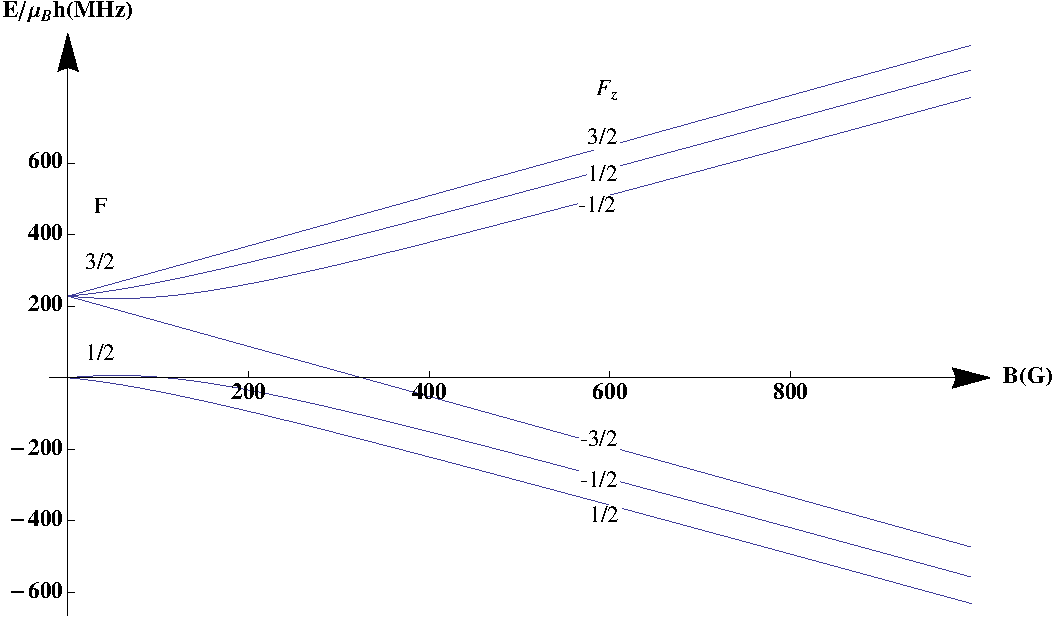
\includegraphics[width=0.8\textwidth]{hyperfineLi6}
\caption{Hyperfine structure of a single \textsuperscript{6}Li atom } 
Levels are marked with $F$ and $F_{z}$ {(see Footnote \ref{foot:intro:f} in page \pageref{foot:intro:f})}
\label{fig:intro:li6}
\end{center}
\end{figure}



\section{Two-body interactions}
Things would be very boring if there was only the single-atom Hamiltonian.  Before we discuss the interaction itself, we introduce one important concept related.   The basic unit with interaction is a pair of atoms.  A ``channel'' is used to refer one  configuration of hyperfine spins for a pair, $\ket{F^{(1)},F_{z}^{(1)}}\otimes\ket{F^{(2)},F_{z}^{(2)}}$  \footnote{Remember that $(F,F_{z})$ are only labels, and do not stand for the total angular momentum unless no magnetic field.\label{foot:intro:f}}    Channels are good basis for non-interaction pair.  A pair of atoms in one channel would stay in it forever if no interaction between them.  Now let us get back to alkali atoms.  Two alkali atoms interact mostly through the overlapping of their electron clouds in the dilute setup.  Thus besides the atom-atom distance, the interaction is mostly a function of electronic spins only, with little-to-none dependence on nuclear spins.  Schematically the interaction can be written as 
\begin{equation}\label{eq:intro:two}
V=f(r)+g(r)\mathbf{S_{1}}\cdot\mathbf{S_{2}}
\end{equation}
The hyperfine levels that diagonalize the single atom Hamiltonian is no longer eigenstates for this interaction.  In another word, the interaction has non-diagonal terms over channels and therefore hybridizes them. Instead, states with definite electronic spins form a good basis for the two-atom interaction.  Nonetheless, most experiments are performed in the so-called high-field region where the electronic spin $S_z$ is approximately a good quantum number, and therefore the original hyperfine levels (channels) serve as a good starting point as the zeroth order.  When the hybridization is considered, multichannel scattering is possible.  The most interesting thing in the multi-channel scattering is resonance.  One of them is Feshbach resonance.  Potential in one channel may be deep enough to sustain a bound-state. When this bound-state energy is close to the zero-energy threshold in the other channel, low-energy scattering properties in that channel is dramatically modified.  This resonance turns out to be extremely useful in   cold atom experiments.  Chapter \ref{sec:intro:twobody} reviews its theory in  two-body physics; the more involving many-body problem is then the central theme of this thesis. 

Let us discuss one example.  In popular experiments setup for $^{6}$Li (Fig. \ref{fig:intro:li6}), usually experiments are prepared with atoms in the two lowest hyperfine levels, described by the  direct product, $\ket{F=\nth{2},F_{z}=-\nth{2}}\otimes\ket{F=\nth{2},F_{z}=+\nth{2}}$.  This is a good approximation until when two atoms are very close.  Recall that the two-atom interaction (Eq. \ref{eq:intro:two}) conserves the z-component of total angular momentum, $F_{z}^{(1)}+F_{z}^{(2)}$.  Therefore this states mixed with four other possible channels, $\ket{\nth{2},-\nth{2}}\otimes\ket{\frac{3}{2},+\nth{2}}$, $\ket{\frac{3}{2},-\nth{2}}\otimes\ket{\nth{2},+\nth{2}}$, $\ket{\frac{3}{2},+\frac{3}{2}}\otimes\ket{\frac{3}{2},-\frac{3}{2}}$, $\ket{\frac{3}{2},+\frac{1}{2}}\otimes\ket{\frac{3}{2},-\frac{1}{2}}$ (All states is labeled as $\ket{F,F_{z}}$).  There are plenty of chances for resonance, and indeed, there are several of them.  Note that close to the resonance, it is normally sufficient to consider only the  channel that is in resonance, while neglect all others.  Another important aspect is whether the two channels share one single hyperfine species (three species in total) or not (four species in total).   The closed channel in the most studied resonance close 834G is approximately $\ket{\frac{3}{2},-\nth{2}}\otimes\ket{\nth{2},+\nth{2}}$ and the resonance is a three-species one\cite{ZhangThesis,ChinRMP}. 

\section{Universality,  the Bethe-Peierls boundary condition, the s-wave scattering length, the two-body density matrix\label{sec:intro:as}}
One important aspect of the interaction in dilute ultracold alkali gas is that for many purposes, it is sufficient to characterize the interaction  by a single two-body parameter, the s-wave scattering length, $a_s$,  because  both the density and the temperature are so low.  Often this is  interpreted as we can replace the real potential with a pseudo potential, $U(\vr)=\frac{4\pi{}a_{s}\hbar^{2}}{m}\delta(\vr)$\cite{pethick, LeggettBEC}.  Nevertheless, an alternative interpretation about $a_s$ is more useful in this work\cite{LeggettBEC, Tan2008-1,Tan2008-2,CombescotTan}.  For the short-range potential, where the potential range, $r_c$, is much smaller than the average interparticle distance, $a_0$, it is not hard to see that in the majority of the time, particles are free-like.  They only interact  when two particles are close to each other.  We can schematically divide the full space into two domains: $\mathcal{D}$, where any two particles are more than $a_c$ away from each other; and otherwise, $\mathcal{I}$. Most physical quantities would be very easy to calculate if only considering the free part, $\mathcal{D}$.  This is almost true in the dilute gas, with modification on a special  boundary condition.  The effect of the potential on wave-function in the short-range region, $\mathcal{I}$, is to enforce the boundary condition on the free part $\mathcal{D}$, $\psi(r)\xrightarrow{r\to0}\psi_{0}(r)$.  For an isometric $\psi_{0}(r)$, the lowest order in radial coordinator $r$ is $\nth{r}$.   Including the next order, a constant,  we have $\psi_{0}(r)=\nth{r}(1-\frac{r}{a_{s}})$ barring the normalization.  All these consideration gives us the simplest non-trivial boundary condition on the radial component of a wave function
\begin{equation}\label{eq:intro:Bethe}
\psi(r)\xrightarrow{r\to0}A\br{\nth{r}-\nth{a_s}}
\end{equation}
which is also known as Bethe-Peierls boundary condition\cite{BethePeierls}.  We neglect all the three-body or more-body interaction, which is a reasonable assumption for the dilute gas. Therefore,  $a_{s}$ is completely determined by two-body physics.  And   this simple boundary condition applies to two-body, few-body, as well as many-body systems, and proves to be a very powerful tool to various problems.  

Eq. \ref{eq:intro:Bethe} coincides the zero-energy s-wave scattering wave function, which explains the name of parameter ``$a_s$'', s-wave scattering length. Nevertheless,   note we did not mention anything about zero energy, where $a_{s}$ is defined in the scattering theory context.  In fact,  this boundary condition applies generally to  any low (positive or negative) energy solutions as long as the energy involved is much lower than the energy scale in the interaction domain $\mathcal{I}$.  Hence this boundary condition can be easily  applied  to close-to-threshold bound state as well.  The s-wave wave function of a weak bound-state is $\psi(r)=\nth{r}e^{-r/a_s}$ in $\mathcal{D}$,\footnote{The extra $\nth{r}$ factor is there for  radial wave function in 3D.} which matches the Bethe-Peierls boundary condition with a positive $a_{s}$ (for  $r\ll{}a_{s}$), and we have the often cited relation for binding energy $E_{b}$.
\begin{equation}
 E_{b}=\frac{\hbar^{2}}{2m_{r}a_{s}^{2}}
\end{equation}
Here $m_{r}$ is the reduced mass for center of mass, which is equal to half of the atom mass for a pair of the same atoms.  This immediately clears one often confusing and counter-intuitive fact, that a positive  $a_s$ corresponds to the bound state.  If interpreting in the normal scattering theory, a positive $a_s$  usually associates with a repulsive interaction, which obviously does not support a bound state.\footnote{This seemingly paradox can be resolved carefully within scattering theory as following. In scattering theory, the fact that  repulsive interaction leads to positive phase shift and therefore positive $a_s$, and attractive interaction leads to negative phase shift and negative $a_s$, is only true when interaction is weak, and phase shift as well as $a_s$ is small.  At the strong interaction, where a bound state is formed, phase shift changes $2\pi$; $a_s$ is large and  changes sign over the threshold. The positive or negative relationship does no longer hold.}

 The s-wave scattering length, $a_s$, or Eq. \ref{eq:intro:Bethe}, does not fix the normalization on the wave function. This normalization factor, encapsulating many-body effects, shows up in many physical quantities.  In a dilute and low-energy system,  its square is proportional to  \emph{integrated contact intensity}, $C$, defined in \cite{ Tan2008-1,Tan2008-2,CombescotTan}, besides a simple constant factor and total density.  At the limit where $a_c\to0$, $C$ and $a_s$ alone, can describe several important physical quantities, (for example internal energy).  A particular useful one for this thesis is the limit at high-momentum distribution of particles, 
 \begin{equation}
 n_k=\frac{C}{k^4}
 \end{equation}
 Note that here \emph{high-momentum} does not mean the absolutely high-momentum, it means lower than the characteristic momentum of potential $1/r_c$, but higher than any other scale, $1/a_0$,...  
 Indeed, when the short-range approximation and low-energy approximation apply, we expect that two-body correlation at  high-momentum ($\gg{k_{F}}$) does not change much from a two-body system to a many-body system.  In this high-energy region, we can always use   the two-body wave function as good approximation. 
 
 In many-body physics, lots of physical observable quantities relate to one set of  quantities, density matrix, $\av{\Psi^\dg\Psi^\dg\cdots\Psi\Psi}$. In fermionic system,  one-body density matrix is often very close to the free case, although the difference can be important for various theories (such as Landau Fermi liquid theory).  A two-body density matrix is often  used for phenomena with  more qualitative difference, such as pairing. Formally, we can decompose a two-body density matrix into orthogonal basis
 \begin{equation}
 \av{\Psi^\dg(x_1)\Psi^\dg(x_2)\Psi(y_2)\Psi(y_1)}=\sum_nC_n\phi_n^\dg(x_1,x_2)\phi_n(y_1,y_2)
 \end{equation}     
 When one or a few $C_n$ is macroscopic, the system behaves quantum mechanically in the macroscopic term.  Especially when only one term is macroscopic, system can often be interpreted as one macroscopic wave function (order parameter).\cite{Leggett}  This can serves as the starting point for several phenomena, such as BEC, BCS superconductor,...
 
Zhang and Leggett developed independently another universality theory based on two-body density matrix \linebreak[2] \cite{shizhongUniv}, which actually takes a more general case than we just discussed.   They asserted that for a short-range potential and low temperature, for example dilute ultracold alkali gas, the basis wave functions $\phi_n$ follows the two-body wave function at short-range. This is actually similar as Bethe-Peierls boundary condition Eq. \ref{eq:intro:Bethe}.  Instead of requiring the simplest form of $\psi_0$ in Eq. \eqref{eq:intro:Bethe}, they require a more general wave-function that solves the  Hamiltonian in two-body level.  And not surprisingly, many physical properties are determined by the normalization factors in boundary condition as using the Bethe-Peierls boundary condition.  

In this thesis, similar idea is used along this line.  We assume the closed-channel correlation follows the its two-body bound-state wave-function in high energy.   However, open-channel does not follow its two-body  wave-function because sensitive nature of resonance. 
 
 
 \chapter{The  Feshbach resonance in two-body physics\label{sec:intro:twobody}}
 As we discussed in Sec. \ref{sec:intro:as}, a two-particle interaction is often approximated by a pseudo-potential characterized with s-wave scattering length $a_{s}$ in a dilute system.   The drastic  change  of $a_{s}$  via tuning energy difference (through a magnetic field) between two channels in the Feshbach resonance gives  experimentalists a rare ability to tune the interaction strength between two particles.  And it is extremely useful to study BEC-BCS crossover where the interaction varies from weak to strong.  
 
Here we briefly review the Feshbach resonance in a two-body system.   As discussed in Chapter \ref{sec:intro:one}, hyperfine level is the eigenstate for isolated single atom.  However, when two atoms interact, most of the interaction comes from  electrons while nucleons interact very little.  Therefore, hyperfine levels is no longer true eigenstates of the two-body system.  Nevertheless, hyperfine level serves a good approximated quantum number and levels are still labelled with it. Furthermore, we take ``channels'' as a pair of hyperfine indices.  Different channels are in general different in interaction strength.  They are decoupled in the lowest order.  In a magnetic field, different channels differ in energy mostly due to the electronic Zeeman energy  as the electronic magnetic moment is much larger than the nuclear magnetic moment.  This energy difference is easy to tune through magnetic field.  

When mixture between channels are taken into consideration, the simple single-channel scattering becomes the multi-channel scattering.  Especially, when the one channel's threshold is close to a bound-state in the other channel, the scattering property in that channel is dramatically altered.  Phase shift can changes $2\pi$ and the s-wave scattering length $a_{s}$ changes to infinity and jumps to the infinity of the opposite sign.  This is essentially what happens in the Feshbach resonance, which was studied by Fano\cite{Fano} and Feshbach \cite{nuclear}  in nuclear and atom physics in 1960s.  Here we  mostly follow treatment in \cite{Leggett} (with some different symbols to comply with the rest of this thesis). 
\footnote{In order to conform with other parts of the thesis, this thesis uses some different symbols comparing to the original works by Leggett \cite{Leggett}.  Here I list them, with the symbols from \cite{Leggett} in parenthesis.  $U$ ($=-V$): open-channel interaction; $V$ ($=-V_{c}$): closed-channel interaction; $Y$ (=-$g\cdot{}f$): inter-channel coupling; $E_{b}$ ($=\epsilon_{0}$):binding energy of closed-channel bound state; $r_{c}$ ($=r_{0}$): range of potential; $\eta$ ($=\epsilon_0+\tilde\delta$) the Zeeman energy difference between two channels; $\mathcal{K}$ ($=\kappa$) see Eq.\ref{eq:intro:kappa}.}

The two-channel Hamiltonian can be written as a $2\times2$ matrix for  the (open,closed) channel
\begin{equation}\label{eq:intro:ham}
\hat{H}(r)=
\begin{pmatrix}
-\frac{\hbar^{2}}{2m_{r}}\nabla^{2}-U(r)&\;&-Y(r)\\
-Y(r)&\;&-\frac{\hbar^{2}}{2m_{r}}\nabla^{2}+\eta-V(r)
\end{pmatrix}
\end{equation}
where the  zero of energy is taken as the energy of two open-channel atoms with infinite separation. $\eta$ is the absolute difference in the Zeeman energy of two channels.  All the interactions are short-range.  For a s-wave solution we have 
\begin{equation}
\psi(r)=\nth{r}\mtrx{\chi(r)\\\chi_{c}(r)}
\end{equation}
Now we can write down the time-independent \sch equation in the radial direction:
\begin{align}
-\frac{\hbar^{2}}{2m_{r}}\chi''-U\chi-Y\chi_c&=E\chi\label{eq:intro:open}\\
-\frac{\hbar^{2}}{2m_{r}}\chi_c''+\eta\chi_c-V\chi_c-Y\chi&=E\chi_c\label{eq:intro:close}
\end{align}
We expand the closed-channel component $\chi_{c}$ over the eigenstates of the isolated closed-channel Hamiltonian, $\chi_{c}=\sum_{i}c_{i}\phi_{i}$, 
\begin{equation}\label{eq:intro:sch2}
-\frac{\hbar^{2}}{2m_{r}}\phi_{i}''-V \phi_{i}=-E_{b}^{(i)}\phi_{i}
\end{equation}
We denote $\phi_{0}$ as the wave function  in resonance and $c_{0}$ as its coefficient.  Here we assume the energy difference between eigenstates, $\phi_{i}$'s, are larger than other energy scales in the problem; hence $c_{0}$ dominates any other $c_{i}$'s.  $\chi_{c}\approx{}c_{0}\phi_{0}$.  Na\"{i}vely speaking, the resonance happens at the point where the closed-channel bound state has the energy exactly at the threshold of the open-channel.  Therefore we introduce the relative detuning, $\tilde\delta=\eta-E_{b}$. Comparing Eq. \ref{eq:intro:open} and Eq. \ref{eq:intro:sch2}, it is not hard to find
\begin{equation}\label{eq:intro:closeCoeff}
\chi_{c}=\frac{\phi_{0}}{E-\tilde\delta}\int{dr'}\,\phi_{0}^{*}(r')Y(r')\chi\br{r'}
\end{equation}
Note that here $\phi_{0}$ is normalized (for radial component).  Put this back to \sch equation of open-channel component $\chi$ (Eq. \ref{eq:intro:open}), 
\begin{equation}\label{eq:intro:chi}
\br{-\frac{\hbar^{2}}{2m_{r}}\frac{d^{2}}{dr^{2}}-U-E}\chi+\frac{1}{E-\tilde\delta}\int_{0}^{\infty}K(r\,r')\chi(r')dr'=0
\end{equation}
where kernel $K(r\,r')$ is
\begin{equation}\label{eq:intro:Krr}
K(r\,r')\equiv\phi_{0}(r)\phi_{0}(r')Y(r')Y(r)\equiv{}K(r'\,r)
\end{equation}
Compare this with the open-channel  \sch equation without coupling to the closed-channel
\begin{equation}\label{eq:intro:chi0}
\br{-\frac{\hbar^{2}}{2m_{r}}\frac{d^{2}}{dr^{2}}-U-E}\chi_{0}=0
\end{equation}
Note that $\chi_{0}(r)\rightarrow0$ as $r\rightarrow0$ and $\chi_{0}(r)\rightarrow{A}(1-r/a_{bg})$ for $r\rightarrow\infty$.\footnote{Note that we are dealing with the internal wave function $\chi_{0}$ here (in region $\mathcal{I}$) instead of the external wave function as in Sec. \ref{sec:intro:as}; therefore, the boundary condition for $r\rightarrow0$ there actually corresponds the boundary condition $r\rightarrow\infty$ here.} Now multiplying Eq. \ref{eq:intro:chi} with $\chi_{0}$ and Eq. \ref{eq:intro:chi0} with $\chi$, integrating from $r=0$ to a  distance much larger than the potential range, $r=r_{0}$, subtracting them, and using Green's theorem, we find 
\begin{equation}
\chi_{0}(r_{c})\chi'(r_{c})-\chi_{0}'(r_{0})\chi(r_{0})+\frac{2m_{r}E}{\hbar^{2}}\int_{0}^{r_{c}}dr\chi_{0}(r)\chi(r)
=\frac{2m_{r}/\hbar^{2}}{E-\tilde\delta}\int_{0}^{r_{0}}dr\int_{0}^{r_{0}}dr'\chi_{0}(r)K(rr')\chi(r')
\end{equation}
Here we can use the boundary condition by let $r\rightarrow\infty$, $\chi_{0}(r)\rightarrow{A}(1-r/a_{bg})$, $\chi(r)\rightarrow\tilde{A}(1-r/a_{s})$.  $Y(r)$ is a short-range interaction and thus $K(r,r')$ only picks the short-range parts of $\chi(r)$ and $\chi_{0}(r)$, which varies little with detuning. Consequently,  the R.H.S approaches a constant.  For the scattering solution at  $E=0$, we have 
\begin{equation}
\nth{a_{s}}-\nth{a_{bg}}=\frac{2m_{r}/\hbar^{2}}{\tilde\delta}\int_{0}^{\infty}dr\int_{0}^{\infty}dr'\chi_{0}(r)K(rr')\chi(r')
\end{equation}
Contrary to the na\"ive intuition, $a_{s}$ does not diverge at the point $\tilde\delta=0$ because of the original interaction in open-channel, $a_{bg}$.  We can define a quantity $\mathcal{K}$, the detuning where $a_{s}$ diverges, by the implicit equation ($\mathcal{K}$ shows up in R.H.S as well)
\begin{equation}\label{eq:intro:kappa}
\mathcal{K}\equiv-\frac{2m_{r}a_{bg}}{\hbar^{2}}\int_{0}^{\infty}{dr}\int_{0}^{\infty}dr'\chi_{0}(r)K(rr')\chi_{\tilde\delta=\mathcal{K}}(r')
\end{equation}
And if we define the ``real detuning'' $\delta\equiv\tilde\delta-\mathcal{K}$, we have 
\begin{equation}
a_{s}(\delta)=a_{bg}\br{1+\frac{\kappa}{\delta}}
\end{equation}
Comparing this with the empirical formula of Feshbach resonance
\begin{equation}
a_{s}(B)=a_{bg}\br{1+\frac{\Delta{B}}{B-B_{0}}}
\end{equation}
We see that $\Delta{B}=\mathcal{K}(\partial\delta/\partial{B})^{-1}$, and $B_{0}$ is the real resonance position.  %Here $\partial\delta/\partial{B}$ is the magnetic momentum difference between two channels.  
\begin{figure}[htbp]
\begin{center}
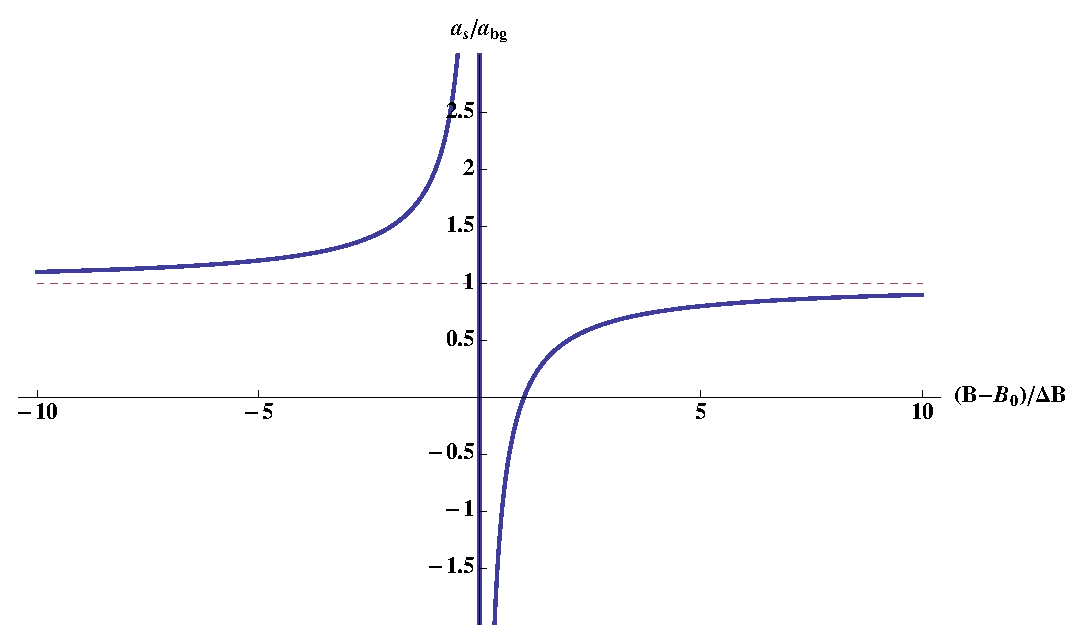
\includegraphics[width=0.8\textwidth]{FeshbachAs}
\caption{S-wave scattering length in Feshbach resonance} 
\label{fig:intro:Feshbach}
{\small Dashed line is $a_{bg}$.}
\end{center}
\end{figure}

Next we consider the bound state \footnote{Here we want to stress the difference between a closed-channel bound-state $\phi_{i}$ and a real bound state with negative energy formed by two channels.   The closed-channel bound state, $\phi_{i}$, is the eigenstate of the  isolated closed-channel Hamiltonian, and is not a real eigenstate for the full two-channel Hamiltonian.  On the other hand, the full  Hamiltonian has bound eigenstates ($E<0$) at large negative detuning (in the two-body context) or BEC-side (in the many-body context).  The bound state solution for a two-channel eigenstate has components both in the open-channel and the closed-channel.  Often the open-channel weight is larger when close to resonance and therefore those bound-states are often called open-channel bound-states.  Only at large negative detuning, the real two-channel bound state is mostly composed of close-channel component, and coincides with close-channel bound-state, $\phi_{i}$ to a large degree.}
where $E<0$, define
\begin{equation}\label{eq:intro:ab}
a_{b}(E)\equiv\frac{\hbar}{(2m_{r}\abs{E})^{1/2}}
\end{equation}
 Here we only study the bound state close to threshold with binding energy much smaller than the binding energy of closed-channel bound state $\phi_{0}$, $\abs{E}\ll{}E_{b}$, and therefore $a_{b}\gg{a_{c}}$.  Outside the range of potential $r_{c}$,  the wave function is proportional to $e^{-r/a_{b}}$. For $r_{c}\ll{}r\ll{}a_{b}$, it can be expanded as  $1-\frac{r}{a_{b}}$, just as the Bethe-Peierls boundary condition (or the s-wave scattering wave function) we discussed in Chapter \ref{sec:intro:as}.  Note that $a_{b}(E)$ is not identified as $a_{s}$ a priori.  We can go through the similar procedure as previous, and it is not hard to find
\begin{equation}
\frac{a_{bg}}{a_{b}}-1=\frac{-\mathcal{K}}{\delta+\mathcal{K}-E}
\end{equation}
Here we assume the short-range part of wave function $\chi$ does not change much and therefore $\mathcal{K}$ stays relatively constant.  Provided both $\delta$ and $\abs{E}$ are much smaller than $\mathcal{K}$, this leads to 
\begin{equation}\label{eq:intro:abKE}
a_{b}=\frac{\mathcal{K}}{\delta-E}
\end{equation}
It is not hard to see that $a_{b}$ indeed \emph{does} coincide with the s-wave scattering length $a_{s}$ when $\abs{E}\ll\abs{\delta}$, and therefore we will use them interchangeably hereafter. This is actually an example our discussion about the Bethe-Peierls boundary condition in Chapter \ref{sec:intro:as}.  Using Eqs. \ref{eq:intro:ab} and \ref{eq:intro:abKE}, it is easy to obtain an equation for $E$
\begin{equation}
(\abs{E}+\delta)^{2}-2\delta_{c}\abs{E}=0
\end{equation}
where $\delta_{c}$ is defined as 
\begin{equation}\label{eq:intro:deltaC}
\delta_{c}\equiv\frac{\mathcal{K}^{2}}{\hbar^{2}/m_{r}a_{bg}^{2}}
\end{equation}
And the solution is  (for $\delta<0$)
\begin{equation}
\abs{E}=\delta_{c}-\delta-\sqrt{\delta_{c}^{2}-2\delta\delta_{c}}
\end{equation}
Furthermore, we can calculate the ``relative weight'' (probability) of closed-channel 
\begin{equation}
\lambda=\br{\frac{1}{E-\tilde\delta}}^{2}\abs{\int{}dr'\phi_{0}(r')Y(r')\chi_{n}(r')}^{2}
\end{equation}
where $\chi_{n}(r)$ is the normalized open-channel bound-state component.  Comparing this with Eq. \ref{eq:intro:kappa}, assuming the short-range part of $\chi_{n}(r)$ does not differ from $\chi_{o}(r)$ much, we can find 
\begin{equation}
\lambda=\nth{(E-\tilde\delta)^{2}}\frac{\hbar^{2}}{2m_{r}a_{bg}}\mathcal{K}a_{b}^{-1}
\end{equation}
For $\abs{\delta}\lesssim\delta_{c}\ll\mathcal{K}$, $E-\tilde\delta\approx\mathcal{K}$ and we have 
\begin{equation}
\lambda=\frac{\hbar^{2}}{2m_{r}a_{bg}}\nth{(\mathcal{K}a_{b})}=\br{\frac{\abs{E}}{2\delta_{c}}}^{1/2}
\end{equation}
Now we can see that  $\delta_{c}$ is a ``characteristic'' energy scale. When $\abs{\delta}\gg\delta_{c}$, $E\approx\delta$, this simply means that when the negative detuning is large, most weight is in the closed-channel, and the real mixed bound state is a closed-channel bound state ($\phi_{0}$) dressed with little open-channel component and therefore the binding energy is roughly equal that of $\phi_{0}$.  The often quoted relation between $a_{s}$ and the binding energy (Eq. \ref{eq:intro:ab}) does not apply here.  On the contrary, when $\abs{\delta}\ll\delta_{c}$, $\abs{E}\approx-\delta^{2}/\delta_{c}\ll\delta$,  and closed-channel weight is much smaller than that of the open-channel, the real bound-state is more or less an open-channel affair with little dress-up from closed-channel.  % It is not hard to  estimate $\delta_{c}$. 

In many-body physics, another important energy scale comes into play, the Fermi energy, $E_{F}$.  When it is much smaller than $\delta_{c}$, i.e. a \emph{broad resonance},  closed-channel has only negligible weight close to resonance, where we are mostly interested in. In such situation, it is a good approximation to take the Feshbach resonance as only a knob to tweak the interaction in the open-channel.  On the contrary, when $E_{F}$ is close even larger than $\delta_{c}$, i.e. a \emph{narrow resonance}, the closed-channel weight can be  significant around resonance, therefore it is required to explicitly take the closed-channel into many-body framework.  










\chapter{The single-channel BEC-BCS crossover\label{sec:intro:1channel}}
In this chapter, we briefly review the BEC-BCS crossover in a single channel.   The idea to describe the BEC and BCS in the same footing stems back several decades \cite{Eagle, LeggettCrossover, Nozieres, RanderiaBEC}.  %One way to interpret BCS is through the existing macroscopic eigenvalue of two-body density matrix (see Sec. \ref{sec:intro:as})\cite{Leggett}.   This eigenvalue corresponds the more familiar anomalous expectation, $\av{a_{\uparrow-\vk}a_{\downarrow\vk}}$.  If simply taking it as wave function of a two-fermion molecule, this eigenfucntion, $\ket{\psi}=(\sum_{\vk}c_{\vk}a^{\dg}_{\uparrow\vk}a^{\dg}_{\downarrow-\vk})\ket{0}$ is very large in size (coherent length), much larger than the average particle distance.  Therefore overlap between different ``molecules'' is significant.   
The BCS theory can be understood as fermions form  ``giant molecules'' and those molecules then condense simultaneously.    It is not hard to show that the famous BCS ansatz is equivalent to  the  coherent state of a two-body pair $\psi^{\dg}=\sum_{\vk}c_{\vk}a^{\dg}_{\uparrow\vk}a^{\dg}_{\downarrow-\vk}$
\begin{equation}\label{eq:intro:BCScoherent}
\prod_{\vk}(u_{vk}+v_{\vk}a^{\dg}_{\uparrow\vk}a^{\dg}_{\downarrow-\vk})\ket{0}=A\exp{}(\sum_{\vk}c_{\vk}a^{\dg}_{\uparrow\vk}a^{\dg}_{\downarrow-\vk})\ket{0}
\end{equation}
where $c_{\vk}=( v_{\vk}/u_{\vk})$. The size of these ``giant molecules'' is in the order of coherent length and much larger than the interparticle distance.
Moving away from the BCS ends, a pair shrinks as the interparticle attraction becomes stronger.  At the BEC side, two-fermion molecules are smaller than the interparticle distance and therefore well-defined. However, the binding energy now is much higher than the typical many-body energy scale and condensation does not happens at the same time when molecules form.  Nevertheless,  at low enough temperature, we can still consider the formation of molecules and their condensation  at the same time, within the same framework as in BCS.  

In the single-channel BEC-BCS crossover model, one images a ``magic'' knob that can tunes the interaction strength along the crossover.  The many-body fermion  system sweeps from fermionic BCS to BEC of diatomic molecules  in response to the interaction change.   This applies directly to the broad-resonance of the two-channel case as well, where the closed-channel weight is negligible and serves only to modify the effective interaction strength in the open-channel.  We mostly follow the path-integral treatment in \cite{RanderiaBEC, Randeria1997, Randeria2008} because it can be readily adapted for two-channel model in the next chapter.
%\subsection{Path integral for one channels}
% !TeX root =thesis.tex
%\subsection{Path integral approach for single channel\label{sec:pathInt}}
\label{sec:pathInt}
Randeria and the company has studied this problem with path integral and it is proved to be a rather nice tool for the problem due to its flexibility and readiness for extension to higher order fluctuation.  

We start with an attractive $\delta$-potential in real space.  This is not equivalent to the l reduced pairing potential as in original BCS work.  However, reduced paring potential only couples  particles of the opposite momentum and does not support simple form of Hubbard-Stratonovich transformation, which is essential to solve the problem in path integral formulation.  
\begin{equation}
\hat{H}-\mu\hat{N}=\sum_{\sigma}\int{d^{d}r}c^{\dagger}_{\sigma}(\vr)\br{-\nth{2m}\nabla^{2}-\mu}c^{}_{\sigma}(\vr)-g\int{d^{d}r}c^{\dagger}_{\uparrow}(\vr)c^{\dagger}_{\downarrow}(\vr)c^{}_{\downarrow}(\vr)c^{}_{\uparrow}(\vr)
\end{equation}
 We can write down the action for the quantum partition function $\mathcal{Z}=\int{D(\bar\psi,\psi)\exp\br{-S[\bar\psi,\psi]}}$
\begin{equation}
S[\bar\psi,\psi]=\int^{\beta}_{0}d\tau\int{d^{d}r}\mbr{\sum_{\sigma}\bar\psi_{\sigma}(\vr,\tau)\br{\partial_{\tau}-\nth{2m}\nabla^{2}-\mu}\psi_{\sigma}(\vr,\tau)-g\bar\psi_{\uparrow}(\vr,\tau)\bar\psi_{\downarrow}(\vr,\tau)\psi^{}_{\downarrow}(\vr,\tau)\psi^{}_{\uparrow}(\vr,\tau)}
\end{equation}
We try to solve this system by introduce Hubbard-Stratonovich transformation.   Introduce a bosonic field $\Delta(\vr,\tau)$ coupled with Cooper channel $\psi(\vr,\tau)\psi(\vr,\tau)$. %Here we follow the normal notation from path integral, $r$ is four tempo-space coordinator.  
We write down first the Gaussian integral of $\Delta$
\begin{equation}
1=\int{D(\bar\Delta,\Delta)}\exp\br{-\nth{g}\int{d\tau{d}^{d}r}\bar\Delta\Delta}
\end{equation}
Note that we absorb the extra constant of integration into the measure of $D(\bar\Delta,\Delta)$.
And with a shift of $\Delta(\vr,\tau)\rightarrow\Delta(\vr,\tau)-g\psi(\vr,\tau)\psi(\vr,\tau)$, we have 
\footnote{$\int{D(\bar\Delta,\Delta)}\cdot1$ is only a constant factor on partition function $\mathcal{Z}$ and has no effect on real physical quantity, therefore, we can take it as 1, (equivalently divide the $\mathcal{Z}$ by a constant)}
\begin{equation}
\exp\br{g\int{d\tau{}d^{d}r}\psi_{\uparrow}\bar\psi_{\downarrow}\psi_{\downarrow}\psi_{\uparrow}}=
\int{D(\bar\Delta,\Delta)}\exp\bbr{-\int{d\tau{d^{d}r}}\mbr{\nth{g}\abs{\Delta}^{2}-\br{\bar\Delta\psi_{\downarrow}\psi_{\uparrow}+\Delta\bar\psi_{\uparrow}\bar\psi_{\downarrow}}}}
\end{equation}
Now the interaction term can be replaced.
\begin{equation*}
\mathcal{Z}=\int{D(\bar\psi,\psi)\int{D(\bar\Delta,\Delta)}\exp\bbr{-\int{d\tau{d^{d}r}}\mbr{\sum_{\sigma}\bar\psi_{\sigma}\br{\partial_{\tau}-\nth{2m}\nabla^{2}-\mu}\psi_{\sigma}+\nth{g}\abs{\Delta}^{2}-\br{\bar\Delta\psi_{\downarrow}\psi_{\uparrow}+\Delta\bar\psi_{\uparrow}\bar\psi_{\downarrow}}}}}
\end{equation*}
This form is bilinear to $\psi$, and we can rewrite it into a nicer form in Nambu spinor representation
\begin{equation}
\bar\Psi=\begin{pmatrix}\bar{\psi}_{\uparrow}&\psi_{\downarrow}\end{pmatrix}\text{,  }\qquad
\Psi=\begin{pmatrix}{\psi}_{\uparrow}\\\bar\psi_{\downarrow}\end{pmatrix}
\end{equation}
\begin{equation}
\mathcal{Z}=\int{D(\bar\psi,\psi)}\int{D(\bar\Delta,\Delta)}\exp
	\bbr{-\int{d\tau{d^{d}r}}\mbr{\nth{g}\abs{\Delta}^{2}-\bar\Psi \nG\Psi}}
\end{equation}
where 
\begin{equation}\label{eq:pathInt:nG}
\nG=\begin{pmatrix}
[\hat{G}_{0}^{(p)}]^{-1}&\Delta\\\bar\Delta&[\hat{G}_{0}^{(h)}]^{-1}
\end{pmatrix}
\end{equation}
is known as Gor'kov Green function, and $[\hat{G}_{0}^{(p)}]^{-1}=-\partial_{\tau}+\nth{2m}\nabla^{2}+\mu$, and $[\hat{G}_{0}^{(h)}]^{-1}=-\partial_{\tau}-\nth{2m}\nabla^{2}-\mu$ represent the non-interacting Green functions of the particle and hole respectively. Now $\Psi$ can be integrated out formally and partition function then only depends on bosonic field $\Delta$.
\begin{equation}\label{eq:pathInt:DeltaPF}
\mathcal{Z}=\int{D(\bar\Delta,\Delta)}\exp
	\bbr{-\mbr{\br{\int{d\tau{d^{d}r}}\nth{g}{\bar\Delta\Delta}}-\ln\det\nG}}
\end{equation}
And action is
\begin{equation}\label{eq:pathInt:DeltaAction}
S[\bar\Delta,\Delta]=
	{\mbr{\br{\int{d\tau{d^{d}r}}\nth{g}{\bar\Delta\Delta}}-\ln\det\nG}}
\end{equation}
Note that $\ln\det\nG$ goes through both the normal space and $2\times2$ Nambu spinor space.  

\subsection{Mean Field Result\label{sec:pathInt:meanfield}}
The saddle point equation of Eq. (\ref{eq:pathInt:DeltaPF}) gives the mean-field result of the system.  First we need to find the derivative of $\ln\det\nG$.  We notice the identity
\begin{equation}
\ln\det\hat{A}=\tr\ln\hat{A}
\end{equation}
and differential rule of a function like $\tr\ln$
\begin{equation}\label{eq:pathInt:diffTr}
\frac{\delta}{\delta\phi_q}\tr\ln(\nG)=\tr(\hat{\mathcal{G}}\frac{\delta}{\delta\phi_q}\nG)
\end{equation}
The saddle equation of Eq. (\ref{eq:pathInt:DeltaPF}) (differential with respect to $\Delta$) is
\begin{equation}
\nth{g}\bar{\Delta}(\vr,\tau)-\tr\mbr{\hat{\mathcal{G}}(\vr,\tau,\vr,\tau)\begin{pmatrix}0&1\\0&0\end{pmatrix}}=0
\end{equation}
Here this matrix is in the Nambu Spinor space.  If we seek a tempo-spacial homogeneous solution of $\Delta_0$, we can find the Nambu Green function from Eq. (\ref{eq:pathInt:nG}) in momentum space
\begin{equation}\label{eq:pathInt:G0}
G_0(p)=\nth{(i\omega_n)^2-E_\vp^2}
\begin{pmatrix}
	i\omega_n+\xi_\vp&-\Delta_0\\
	-\bar{\Delta}_0&i\omega_n-\xi_\vp
\end{pmatrix}
\end{equation}
Here $\omega_n$ is Matsubara frequency of Fermions.  $\xi_{\vk}=\epsilon_{\vk}-\mu$, $\epsilon_{\vk}=\vk^{2}/2m$,  $E_\vp=\sqrt{\xi_\vp^2+\abs{\Delta_0}^2}$.  And the saddle point equation can be rewritten as 
\begin{equation}
\nth{g}\bar{\Delta}_0=\frac{T}{L^d}\sum_{\vp,n}\frac{\bar\Delta_0}{\omega_n^2+E_\vp^2}
\end{equation}
The summation of Matsubara frequency can be evaluated and we find 
\begin{equation}
\nth{g}=\nth{L^d}\sum_{\vp}\frac{1-2n_f(E_p)}{2E_p}=\nth{L^d}\sum_{\vp}\frac{\tanh{(E_p/2T)}}{2E_p}
\label{eq:pathInt:gap}
\end{equation}
where $n_f(\epsilon)$ is the fermi distribution function.  This is exactly the gap equation obtained from other methods as well.  On the other hand, $\nG$ in Eq. (\ref{eq:pathInt:nG})  is the inverse of fermion-fermion correlation of $\Psi$.  In mean field, $G_{0}$ as Eq. (\ref{eq:pathInt:G0}) can be diagnosed in momentum space with a canonical (Bogoliubov) transformation.  Nevertheless, poles is where  $\omega^2-E_\vp^2=0$ (with a analytic continue of $i\omega_{n}\rightarrow\omega+0^{+}$) as we can see from  Eq. (\ref{eq:pathInt:G0}) and therefore the spectrum of fermionic excitation is $\pm{}E_{p}$.  

Summand in Eq. \ref{eq:pathInt:gap} does not decreases fast enough in 3D and the summation does not converges.  This is because our assumption of contact interaction breaks down when reaching real potential range $a_{c}$, i.e., the summation of momentum is capped at some high momentum $\Lambda$ related to $1/a_{c}$.  Notice that in 3-D, we have a relation that connect the bare potential $g$ to more physically observable s-wave scattering length $a_{s}$
\begin{equation}\label{eq:pathInt:as}
\frac{m}{4\pi{}a_{s}}=-\nth{g}+\sum_{k<\Lambda}\nth{2\epsilon_{\vk}}
\end{equation}
We can renormalize Eq. \ref{eq:pathInt:gap} with this relation
\begin{equation}
-\frac{m}{4\pi{}a_{s}}=\sum_{\vk}\mbr{\frac{\tanh{(E_k/2T)}}{2E_k}-\nth{2\epsilon_{\vk}}}
\end{equation}
Now the gap equation has proper decay in high momentum and no artificial cutoff is necessary.  There are two unknown parameters, $\mu$ and $\Delta$,  in the equation.  We need another equation in order to pin them down. To compliment the gap equation, we can introduce the number equation, $n=-\partial\Omega/\partial\mu$. At the saddle point, the thermodynamic potential is $\Omega_{0}=S[\Delta_{0}]/\beta$, and we have number equation
\begin{equation*}
n=-\nth{\beta}\tr\br{{G_{0}\pdiff{G_{0}^{-1}}{\mu}}}
\end{equation*}
similarly the summation over the Mastubara frequency can be evaluated and we have equation
\begin{equation}
n=\nth{L^{d}}\sum_{\vk}\mbr{1-\frac{\epsilon_{\vk}}{E_{\vk}}\tanh{(\frac{E_{\vk}}{2T})}}
\end{equation}

\subsection{Gaussian fluctuation and collective mode}\label{sec:collective1}
Once the mean field value is obtained, we can expand partition function Eq. (\ref{eq:pathInt:DeltaPF}) around it ($\Delta(\vr,\tau)=\Delta_{0}+\eta(\vr,\tau)$). The linear order of  expansion is zero because $\Delta_{0}$ is the saddle point.  The next order gives us the bilinear terms on $\eta$, i.e., correlation of bosonic field $\Delta$ (four-fermion correlation).  Note that here the hamiltonian only has an extreme-short-range ($\delta$) potential, therefore it cannot cover the situation of charged system where long-range Columnb interaction cannot be neglected.  We will discuss this later.  Nevertheless, it is conceivable that a more realistic short-range potential only renormalizes some parameters in the following calculation while leaves the qualitative result unmodified.  

Notice that we can expand the second term in Eq. \ref{eq:pathInt:DeltaPF} for $\hat{G}{}^{-1}=\hat{G}_{0}^{-1}+\hat{K}$
\begin{equation}\label{eq:pathInt:expand}
\tr\ln \hat{G}^{-1}=\tr\ln\hat{G_{0}}^{-1}+\tr(\hat{G_{0}}\hat{K})-\nth{2}\tr(\hat{G_{0}}\hat{K}\hat{G_{0}}\hat{K})+\cdots
\end{equation}
In our case,
\begin{equation}
\hat{K}=\begin{pmatrix}
0&\eta\\
\eta^{*}&0
\end{pmatrix}
\end{equation}
Here the linear terms of $\hat{K}$ or $\eta$ ($\eta^{*}$) are zero as the saddle point condition.  So to the second order, the action is 
\begin{equation}\label{eq:pathInt:DeltaActionGaussian}
S[\Delta_{0},\eta,\eta^{*}]=S[\Delta_{0}]+
	\nth{2g}\tr(\hat{K}\hat{K})+\nth{2}\tr(\hat{G_{0}}\hat{K}\hat{G_{0}}\hat{K})
\end{equation}
Write the last term into the momentum representation
\begin{equation}
\tr(\hat{G_{0}}\hat{K}\hat{G_{0}}\hat{K})=\sum_{q,p}\Tr\br{G_{0}({p})K_{q}G_{0}{}({p-q})K_{-q}}
\end{equation}
Notice that the second ``$\Tr$'' and following ``$\Tr$'' in this section only runs in Nambu spinor space and $q={(\vq,q_{l})}$, $p=(\vp,p_{n})$ are all four momentum, where $q_{l}$ is bosonic Matsubara frequency while $p_{n}$ is fermionic Matsubara frequency.
\begin{equation}
K_{q}=\begin{pmatrix}
0&\eta_{q}\\
\eta^{*}_{-q}&0
\end{pmatrix}
\end{equation}
If we introduce the a new vector 
\begin{equation}
\eta{(q)}=\begin{pmatrix}\eta_{q}\\\eta^{*}_{-q}\end{pmatrix}\qquad
\eta^{\dg}{(q)}=\begin{pmatrix}\eta^{*}_{q}&\eta_{-q}\end{pmatrix}
\end{equation}
the action can be rewritten into a more compact form
\begin{equation}
S[\Delta_{0},\eta,\eta^{*}]=S[\Delta_{0}]+\nth{2}\sum_{q}\Tr\mbr{\eta^{\dg}(q)\mathbf{M(q)}\eta(q)}
\end{equation}
Notice that we can always choose a real $\Delta_{0}$ and therefore $G_{0}{\ _{12}}(p)=G_{0}{\ _{21}}(p)$, we have 
\begin{equation}
\mathbf{M(q)}=
\begin{pmatrix}
\nth{g}+\sum_{p}G_{0}{\ }_{11}(p)G_{0}{\ }_{22}(p-q)&\sum_{p}G_{0}{\ }_{12}(p)G_{0}{\ }_{12}(p-q)\\
\sum_{p}G_{0}{\ }_{12}(p)G_{0}{\ }_{12}(p-q)&\nth{g}+\sum_{p}G_{0}{\ }_{11}(p-q)G_{0}{\ }_{22}(p)
\end{pmatrix}
\end{equation}
The summation over (fermionic) Matsubara frequency of $p_{n}$ can be carried out at zero temperature
\footnote{\label{foot:intro:sum}The summation of Matsubara frequency of function $h(i\omega_{n})$ is carried out by the normal method to multiplying $h(z)$ with fermi distribution function $n_{F}(z)$, and then find all residues with a contour over infinity.  However, due to zero temperature, the  $n_{F}(z)$ only nonzero at the negative singular points of $h(z)$, $-E_{\vk}$ in our case.  (The other singular point $E_{\vk}$ gives $n_{F}(E_{\vk})=0$ for zero temperature.}
\begin{equation}
\begin{split}
M_{11}(q)&=M_{22}(-q)\\
	&=\nth{g}+\sum_{\vp{,}p_{n}}G_{0}{\ }_{11}(p)G_{0}{\ }_{22}(p-q)\\
	&=\nth{g}+\sum_{\vp}\br{\frac{u^{2}u'^{2}}{iq_{l}-E-E'}-\frac{v^{2}v'^{2}}{iq_{l}+E+E'}}
\end{split}
\end{equation}
\begin{equation}
\begin{split}
M_{12}(q)&=M_{21}(q)\\
	&=\sum_{\vp{,}p_{n}}G_{0}{\ }_{12}(p)G_{0}{\ }_{12}(p-q)\\
	&=\sum_{\vp}uvu'v'\br{\nth{iq_{l}+E+E'}-\nth{iq_{l}-E-E'}}
\end{split}
\end{equation}
where $u=u_{\vp}$, $v=v_{\vp}$, $E=E_{\vp}$ and $u'=u_{\vp-\vq}$, $v'=v_{\vk-\vq}$, $E'=E_{\vk-\vq}$.  $u$, $v$, $E$ are as defined usually in BCS literature. 
\begin{equation}
v_{\vk}^{2}=1-u_{\vk}^{2}=\nth{2}\br{1-\frac{\xi_{\vk}}{E_{\vk}}}
\end{equation}
 The $G^{(M)}=\mathbf{M}^{-1}$ is the correlation function of $\eta$ (or $\Delta$) and its poles give the spectrum of collective mode as every  $\eta_{q}$ (or $\Delta_{q}$) involves many fermions moving in a coherent manner.  So the spectrum of collective modes can be determined by $\det{M(\omega,\vq)}=0$ after we analytically continue for the frequency $iq_{l}\rightarrow\omega+i0^{+}$.  
 
For low energy modes, where $\omega,\,\abs{\vq}^{2}\ll\min\bbr{E_{\vk}}$ both are much smaller than $\Delta_{0}$, we can expand $M$ with $\omega$ and $\vq$.  


\subsection{Alternative in inverting green function\label{sec:diagonalizeGreen1}}
In the above section, we have inversion of Gorkov green function Eq. (\ref{eq:pathInt:nG}) and it can be invert easily as Eq. (\ref{eq:pathInt:G0}).   Alternatively, we can use a different approach which proves to be more convenient in two-channel problem.  First, we diagonalize $\nG$ with unitary transformation $T$, in momentum space
\begin{equation}
\nG=\mtrx{i\omega_{n}-\xi_{k}&\Delta\\\bar\Delta&i\omega_{n}+\xi_{k}}=T^{\dg}BT
\end{equation}
It is easy to show that such $T$ and $B$ satisfing above equation are
\begin{equation}
T=\mtrx{u_{k}&v_{k}\\-v_{k}^{*}&u_{k}}\qquad{}B=\mtrx{i\omega_{n}+E_{k}&0\\0&i\omega_{n}-E_{k}}
\end{equation}
where $u_{k}^{2}(v_{k}^{2})=\nth{2}(1\pm\xi_{k}/E_{k})$ and $E_{k}$ are conventionally defined quantities in BCS theory.   Actually, this transformation is nothing but Bogoliubov canonical transformation, and $B$ matrix simply describes spectrum of fermionic quasi-particles.  Now it is easy to invert $\nG$
\begin{equation}
G=T^{\dg}B^{-1}T
\end{equation}
Green's function $G$ takes a more conventional form $A/(i\omega_{n}-e_{k})$ without any dependency on frequency in nominator as Eq. (\ref{eq:pathInt:G0}). Matsubara frequency summation over $G_{0}(k)$ in mean-field and $G_{0}(k)G_{0}(k+q)$ in Gaussian order are then fairly straight-forward as in text-book.  




\begin{subappendices}
\end{subappendices}


%\chapter{Path-Integral approach}


% !TeX root =thesis.tex

\chapter{Path integral approach for two-channel\label{ch:path2}}
For narrow resonance, atoms have considerable weight in close-channel and the Pauli exclusion between two channels cannot be neglected.  A many-body framework needs to include both channels.  Path integral approach is particular suitable for crossover problem.   The Hubbard-Stratonovich transformation is powerful tool to study non-trivial degree of freedom (order parameter) in the system.  It is more or less equivalent to other approaches at mean-filed level (Appendix \ref{ch:mean}). But it has great advantage to be easily extended to explore the fluctuation over the mean-field result.  

For two-channel problem, we write down the Hamiltonian as
\begin{equation}\label{eq:pathInt2:ham2}
\begin{split}
H&=\int{d^{d}r}\bigg\{\sum_{j}\bar\psi_{j}\mbr{\nth{2m}(-i\nabla)^{2}-\mu+\eta_{j}}\psi_{j}\\
	&\qquad-U\bar\psi_{a}(r)\bar\psi_{b}(r)\psi_{b}(r)\psi_{a}(r)-V\bar\psi_{a}(r)\bar\psi_{c}(r)\psi_{c}(r)\psi_{a}(r)\\
	&\qquad-\mbr{Y\bar\psi_{a}(r)\bar\psi_{b}(r)\psi_{c}(r)\psi_{a}(r)+h.c.}
	\bigg\}\\
 &=\int{d^{d}r}\bigg\{\sum_{j}\bar\psi_{j}\mbr{\nth{2m}(-i\nabla)^{2}-\mu+\eta_{j}}\psi_{j}
 	-(\bar\psi\bar\psi)\mtrx{U&Y\\Y^{*}&V}(\psi\psi)
\end{split}
\end{equation}
Here $\eta_{j}$ is the Zeeman energy of the specific hyperfine species.  ``a'' is the common species of two channels, (a,b) is the open channel and (a,c) is the close channel.  All the interactions ($U$, $V$, $Y$), are contact type, this simplifies Hubbard-Stratonovich transformation considerably.  It is plausible as we only study low-energy phenomenon for the short-range potential.   

We can introduce a unitary transformation $Q$ (mixing two channels) to diagonalize the interaction matrix into diagonal matrix $A$.
\begin{equation}
\begin{split}
Q^{\dg}AQ=\mtrx{U&Y\\Y^{*}&V}\equiv{}\tilde{U}\\
\tilde{U}\equiv\mtrx{U&Y\\Y^{*}&V}=Q\mtrx{A_{11}&0\\0&A_{22}}Q^{\dg}
\end{split}
\end{equation}
The finite temperature action is 
\begin{equation}\label{eq:pathInt2:actionFermi}
S(\bar\psi,\psi)=\int^{\beta}_{0}d\tau\int{d^{d}r}\mbr{\sum_{j}\bar\psi_{j}(\partial_\tau-\nth{2m}\nabla^{2}-\mu+\eta_{j})\psi_{j}
-(\bar\psi\bar\psi)Q^{\dg}AQ(\psi\psi)}
\end{equation}

Now $(\psi\psi)$ is column vector and $(\bar\psi\bar\psi)$ is row vector
\begin{equation*}
(\bar\psi\bar\psi)=\mtrx{\bar\psi_{a}\bar\psi_{b}&\bar\psi_{a}\bar\psi_{c}}
\qquad(\psi\psi)=\mtrx{\psi_{b}\psi_{a}\\\psi_{c}\psi_{a}}
\end{equation*}

Similar as in Sec. \ref{sec:pathInt}, we can make Hubbard-Stratonovich transformation on the action.   Here, introduce a bosonic field as a 2-component vector   and start from a fat identity \cite{Altland}
\begin{equation}\label{eq:pathInt2:indetity}
1=\int{D(\Delta,\bar\Delta)}\exp(-\int{dx}\Delta^{\dg}A^{-1}\Delta)
\end{equation}
\[
\Delta^{\dg}=(\bar\Delta_{1},\bar\Delta_{2})\qquad\Delta=\begin{pmatrix}\Delta_{1}\\\Delta_{2}\end{pmatrix}
\]
here $x$ is four-coordinator,  $\int{dx}=\int^{\beta}_{0}d\tau\int{d^{d}r}$.  All the integral constant is absorbed into measure of functional integral of $D(\Delta,\bar\Delta)$.


We can make a shift in $\Delta$
\begin{equation}
\Delta\longrightarrow\Delta-A\,Q(\psi\psi)
\end{equation}
Write it into the matrix form
\begin{equation*}
\mtrx{\Delta_{1}\\\Delta_{2}}\longrightarrow
	\mtrx{\Delta_{1}\\\Delta_{2}}-\mtrx{A_{11}&0\\0&A_{22}}\mtrx{Q_{11}&Q_{12}\\Q_{21}&Q_{22}}
	\mtrx{\psi_{b}\psi_{a}\\\psi_{c}\psi_{a}}
\end{equation*}
\begin{equation*}
\mtrx{\bar\Delta_{1},\bar\Delta_{2}}\longrightarrow
	\mtrx{\bar\Delta_{1},\bar\Delta_{2}}-
	\mtrx{\bar\psi_{a}\bar\psi_{b}&\bar\psi_{a}\bar\psi_{c}}
	\mtrx{Q_{11}^{*}&Q_{21}^{*}\\Q_{12}^{*}&Q_{22}^{*}}\mtrx{A_{11}&0\\0&A_{22}}
\end{equation*}

Note that in principle, $\bar{\Delta}_{i}$ is not simple complex conjugate of $\Delta_{i}$ as they are related to fermion field $\psi$ and $\bar\psi$, which are both Grassman numbers and is not relevant to each other.  But in our solution (to the level of mean-field as well as simple Gaussian level of collective mode), we actually take them as complex conjugate.  Now the fat identity Eq. \ref{eq:pathInt2:indetity} becomes 
\begin{equation}
1=\int{D(\Delta,\bar\Delta)}\exp\big\{-\int{dx}
	[\Delta^{\dg}A^{-1}\Delta-(\bar\psi\bar\psi)Q^{\dg}\Delta-\bar\Delta{Q}(\psi\psi)+(\bar\psi\bar\psi)Q^{\dg}AQ(\psi\psi)]\big\}
\end{equation}
And we have 
\begin{equation}
\exp[\int{dx}(\bar\psi\bar\psi)Q^{\dg}AQ(\psi\psi)]
=\int{D(\Delta,\bar\Delta)}\exp\big\{-\int{dx}
	[\Delta^{\dg}A^{-1}\Delta-(\bar\psi\bar\psi)Q^{\dg}\Delta-\bar\Delta{Q}(\psi\psi)]\big\}
\end{equation}
This is ready to be apply to the original action in Eq. \ref{eq:pathInt2:actionFermi}, 
\begin{equation}\label{eq:pathInt2:actionMix}
S_{\tau}(\bar\Delta,\Delta,\bar\psi_{i},\psi_{i})=\int^{\beta}_{0}d\tau\int{d^{d}r}\bbr{\sum_{j}\bar\psi_{j}(\partial_\tau-\nth{2m}\nabla^{2}-\mu+\eta_{j})\psi_{j}
+[\Delta^{\dg}A^{-1}\Delta-(\bar\psi\bar\psi)Q^{\dg}\Delta-\bar\Delta{Q}(\psi\psi)]}
\end{equation}
We can introduce a spinor space similar to Nambu spinor representation in single-channel superconductivity.  
\begin{equation}
\bar\Psi=\mtrx{\bar\psi_{a}&\psi_{b}&\psi_{c}}\qquad\Psi=\mtrx{\psi_{a}\\\bar\psi_{b}\\\bar\psi_{c}}
\end{equation}
the action can be rewritten in a more compact form
\begin{equation}\label{eq:pathInt2:actionMix}
S(\bar\Delta,\Delta,\bar\psi_{i},\psi_{i})=\int^{\beta}_{0}d\tau\int{d^{d}r}
	\mbr{\Delta^{\dg}A^{-1}\Delta-\bar\Psi\mathcal{G}^{-1}\Psi}
\end{equation}
where 
\begin{equation}
\mathcal{G}^{-1}=
\begin{pmatrix}
-\partial_{\tau}+\nth{2m}\nabla^{2}+\mu-\eta_{a}&Q^{*}_{11}\Delta_{1}+Q^{*}_{21}\Delta_{2}&Q^{*}_{12}\Delta_{1}+Q^{*}_{22}\Delta_{2}\\
Q^{}_{11}\bar\Delta_{1}+Q^{}_{21}\bar\Delta_{2}&-\partial_{\tau}-\nth{2m}\nabla^{2}-\mu+\eta_{b}&0\\
Q^{}_{12}\bar\Delta_{1}+Q^{}_{22}\bar\Delta_{2}&0&-\partial_{\tau}-\nth{2m}\nabla^{2}-\mu+\eta_{c}
\end{pmatrix}
\end{equation}
The action is now bilinear to $\Psi$ and we can integrate it out formally
\begin{equation}
S(\bar\Delta,\Delta)=\int{dx}
	\br{\Delta^{\dg}{}A^{-1}\Delta-\tr\ln{G}^{-1}}
\end{equation}
This form can be simplified by introducing mixture within two channels.
\begin{equation}\label{eq:pathInt2:Ddef}
D\equiv\mtrx{D_{1}\\D_{2}}=Q^{\dg}\Delta
\end{equation}
It is not difficult to see that $D$ actually describe the off-diagonal coupling in fermionic field $\Psi$ and is the counterpart of order parameter, gap, in single-channel problem instead of $\Delta$ here.  We will see it  more clearly when  discussing mean-field solution. 

We furthermore assume $\eta_{a}=\eta_{b}=0$, $\eta_{c}=\eta$. (i.e., $\eta$ is the absolute Zeeman energy difference of two channels.) In frequency-momentum space, 
\begin{equation}\label{eq:pathInt2:nG}
\mathcal{G}^{-1}=i\omega_{n}I+
\begin{pmatrix}
-\xi_{k}&D_{1}&D_{2}\\
\bar{D}_{1}&+\xi_{k}&0\\
\bar{D}_{2}&0&+\xi_{k}+\eta
\end{pmatrix}
\end{equation}
here $\xi_{k}=\nth{2m}k^{2}-\mu$; and 
\begin{equation*}
\bar\Delta=\bar{D}\,Q^{\dg}\qquad\Delta=Q\,D
\end{equation*}
\[
\bar\Delta{}A^{-1}\Delta=\bar{D}Q^{\dg}A^{-1}QD=\bar{D}\tilde{U}^{-1}D
\]
Now we can change the functional variable into $D(\bar{D})$ 
\begin{equation}\label{eq:pathInt2:actionD}
S(\bar{D},D)=\int{dx}\br{\bar{D}\tilde{U}^{-1}D-\tr\ln{G}^{-1}}
\end{equation}




\section{Diagonalize Green's function, Fermionic mode and Bogoliubov transformation\label{sec:diagonalGreen}}
Here we use the approach in Sec. \ref{sec:diagonalizeGreen1} for our problem.  In current problem, we need to diagonalize a $3\times3$ matrix Eq. \ref{eq:pathInt2:nG}, in another word, we need to figure out the Bogoliubov canonical transformation over the spiner representation and the quasiparticle spectrum for this problem.   This involves solving a cubic equation. An exact solution exists in principle.  However,  it offers little intuition in writing the exact result, instead we  find that  spectrum from the broad-resonance, where the only effect of close-channel is to modify the effective interaction of open-channel, serves a reasonable lowest order approximation and we proceeds to find the first order of correction over it (See Appendix \ref{sec:diagonalize} and \ref{sec:pathApp:consistency}). 


Within the assumption that spectrum  deviates not too much from na\"{i}ve broad-resonance solution, we  break down the unitary transformation into two steps $T$ and $L$. 
\begin{equation}\label{eq:pathInt2:B}
B_k=L_k^{\dg}T_k^{\dg}G_k^{-1}T_kL_k
\end{equation} 
Here $T$ and $L$ are both unitary transformation.  We take $T$ as the transformation at lowest order, i.e., when we can ignore Pauli exclusion between channels. 
\begin{equation}
T_k=\mtrx{u_k&v_k&0\\-v_k&u_k&0\\0&0&1}
\end{equation}
Here we define 
\begin{gather}
v_{\vk}^{2}\equiv1-u_{\vk}^{2}\equiv\nth{2}\br{1-\frac{\xi_{\vk}}{E_{\vk}}}\\
E_{\vk}\equiv(\xi_{\vk}^{2}+D_{1}^{2})^{1/2}
\end{gather}

In the broad-resonance, where only the BCS pairing in open channel needs to be considered, $T$ is enough to diagonalize $G^{-1}$ and $L$ is simply identity matrix.  %Here we will try to approximate it to the first order correction due to Pauli exclusion between two-channel.  
In the narrow resonance, $T$ cannot diagonalize $G^{-1}$ because of the Pauli exclusion between channels and therefore $L$ stands the extra correction due to Pauli exclusion in the canonical transformation. Basically, we seek the solution around the BCS ansatz ($T$ transform). 
Apply $T$ onto $G^{-1}$, we have 
\begin{equation}\label{eq:pathInt2:G2}
T_k^{\dg}G_k^{-1}T_k=i\omega_nI+\mtrx{-E_k&0&u_kD_2\\0&+E_k&v_kD_2\\u_kD_2&v_kD_2&+\xi_k+\eta}
\end{equation}
We regard the off-diagonal elements as perturbation.  This matrix can then be diagonalized with another unitary transformation $L_{\vk}$ within the first order of $D_{2}^{2}/(E\eta)$  (Please see Appendix \ref{sec:diagonalize} for details.)
\begin{equation}
\begin{split}
B_{\omega_{n},\vk}&=i\omega_{n}I-
	\mtrx{\xi_{1}{}_{\vk}&0&0\\0&-\xi_{2}{}_{\vk}&0\\0&0&-\xi_{3}{}_{\vk}}\\
	&\approx{}i\omega_{n}I+
	\mtrx{-E_{\vk}-\frac{D_{2}^{2}u_{\vk}^{2}}{\eta}&0&0\\
	0&E_{\vk}-\frac{D_{2}^{2}v_{\vk}^{2}}{\eta}&0\\0&0&\xi_{\vk}+\eta+\frac{D_{2}^{2}}{2\eta}}
%	&=
%	\mtrx{i\omega_{n}-E_{\vk}&0&0\\0&i\omega_{n}+E_{\vk}&0\\0&0&i\omega_{n}+\eta}
%	+\mtrx{-\frac{D_{1}^{2}}{\eta}&0&0\\0&-\frac{D_{2}^{2}}{\eta}&0\\0&0&+\frac{D_{1}^{2}+D_{2}^{2}}{2\eta}}\\
%	&\equiv{}B^{(0)}_{\vk}+B^{(1)}_{\vk}
\end{split}	
\end{equation}
Here we choose the sign of $\xi_{1,2,3}$  to make their zeroth order positive.  
we have 
\begin{align}\label{eq:pathInt2:xiExpand}
\xi_{1\vk}&\approx{}E_{\vk}+\frac{D_{2}^{2}u_{\vk}^{2}}{\xi_{\vk}+\eta}&\equiv{}&E_{\vk}+\gamma_{1\vk}\\
\xi_{2\vk}&\approx{}E_{\vk}-\frac{D_{2}^{2}v_{\vk}^{2}}{\xi_{\vk}+\eta}&\equiv{}&E_{\vk}+\gamma_{2\vk}
\label{eq:pathInt2:xiExpand2}\\
\xi_{3\vk}&\approx{}\xi_{\vk}+\eta-\frac{D_{2}^{2}}{2(\xi_{\vk}+\eta)}&\equiv{}&\xi_{\vk}+\eta+\gamma_{3\vk}
\label{eq:pathInt2:xiExpand3}
\end{align}

\begin{equation}\label{eq:pathInt2:L1}
L_{\vk}\approx{}I+
\mtrx{0&-\frac{D_{1}{}D_{2}{}}{4E^{2}_{\vk}}&u_{\vk}\\
\frac{D_{1}{}D_{2}{}}{4E^{2}_{\vk}}&0&v_{\vk}\\
-u_{\vk}&-v_{\vk}&0
}\frac{D_{2}{}}{\eta}
\equiv{}I+\delta_{k}\qquad
L^{\dg}_{\vk}=I-\delta_{\vk}
\end{equation}
Here we use $uv=D_{1}/2E$.    Note that $L$ and $L^{\dg}$ are unitary only to the first order of $D_{i}/\eta$
And now it is easy to express the Green's function
\begin{equation}
G_{\vk}=T_{\vk}L_{\vk}B_{\vk}^{-1}L_{\vk}^{\dg}T_{\vk}^{\dg}
\end{equation}
This is ready to be expanded over the perturbation in order of  $D_{2}^{2}/(E\eta)$ or $D_{i}/\eta$.  It is easy to see that all $\omega_{n}$ dependence concentrates on $B_{\vk}$, which is linear in $\omega_{n}$  and simplifies the Matsubara frequency summation considerably.   
\begin{subequations}\label{eq:pathInt2:Gexpand}
\begin{gather}
G_{k}\approx{}T_{\vk}B_{\omega_{n},\vk}^{-1}T_{\vk}^{\dg}+T_{\vk}\delta_{\vk}B_{\omega_{n},\vk}^{-1}T_{\vk}^{\dg}
	-T_{\vk}B_{\omega_{n},\vk}^{-1}\delta_{\vk}T_{\vk}^{\dg}
	\equiv{}G_{\vk}^{(0)}+G_{\vk}^{(1)}\\
	G_{\vk}^{(0)}=T_{\vk}B_{\omega_{n},\vk}^{-1}T_{\vk}^{\dg}\\
	G_{\vk}^{(1)}=T_{\vk}\delta_{\vk}B_{\omega_{n},\vk}^{-1}T_{\vk}^{\dg}
	-T_{\vk}B_{\omega_{n},\vk}^{-1}\delta_{\vk}T_{\vk}^{\dg}
\end{gather}
\end{subequations}
\subsection{Fermionic mode and Bogoliubove transformation}
In fact, if we limit ourselves in mean field level, we can interpret the above transform $T_\vk{}L_\vk$ as Bogoliubov canonical transformation and $B$ gives us spectrum of fermionic quasi-particle excitation.  At mean field, both $D_{1}$ and $D_{2}$ are taken as constants. Furthermore, they are taken as real.  From Eqs. (\ref{eq:pathInt2:xiExpand}-\ref{eq:pathInt2:xiExpand3}), we see that the fermionic excitation modes basically follow the pattern in broad resonance.  In broad resonance where close channel only modifies the interaction in open channel,  there are basically two quasi-particle modes: Bogoliubov quasi-particle mdoe in open channel, $E_{\vk}=\sqrt{\xi^{2}_{\vk}+D_{1}^{2}}$; and the high normal fermi excitation mode in close-channel, $\xi_{\vk}+\eta$.  In narrow resonance, first of all, the gap $D_{1}$ is the modified  by consideration of extra Pauli exclusion.  Once that is taken into account, the above conclusion is still correct except high-order correction in $D_{2}^{2}/\eta$.   From Eq. \ref{eq:pathInt2:actionMix} and Eq. \ref{eq:pathInt2:B}, the action is diagonal for $\Phi_\vk=L^{\dg}_{\vk}T^{\dg}_{\vk}\Psi_{\vk}$, which indicate $L^{\dg}_{\vk}T^{\dg}_{\vk}$ is closely related to Bogoliubov canonical transformation and quasi-particles.  
\begin{equation}
\end{equation}




%We only need to keep the zeroth order term for $B_{\vk}^{-1}$ for first order expansion.  
\section{Mean field equation \label{sec:pathInt2:meanfield}}
Use the same techniques as Eq. (\ref{eq:pathInt:diffTr}), we have two saddle point equations for $D_{1}$ and $D_{2}$,
 \begin{align}
\frac{\delta}{\delta{}D_{1}}:&\qquad&
(\tilde{U}^{-1})_{11}\bar{D}_{1}+(\tilde{U}^{-1})_{21}\bar{D}_{2}-\tr\mbr{{G_{0}}\cdot\cmtrx{0&1&0\\0&0&0\\0&0&0}}=0
\label{eq:pathInt2:mf01}\\
\frac{\delta}{\delta{}D_{2}}:&\qquad&
(\tilde{U}^{-1})_{12}\bar{D}_{1}+(\tilde{U}^{-1})_{22}\bar{D}_{2}-\tr\mbr{{G_{0}}\cdot\cmtrx{0&0&1\\0&0&0\\0&0&0}}=0
\label{eq:pathInt2:mf02}
 \end{align}
 
 
  If we take $D$ as real constant,
  %\footnote{Actually $D_{2}{_{\vk}}$ cannot be constant at high momentum.  However, for the momentum we are interested, i.e. the momentum lower or in the order of Fermi momentum, it slowly varies.  Therefore  it is reasonable to take it as constant.}     
  we can find the mean field result. Eq. (\ref{eq:pathInt2:nG}) can be inverted to get $G$.  The inversion is quite tedious, but fortunately, we only need two elements of the $G$ matrix ($G_{0\, (21)}$ and $G_{0 \,(31)}$).  The final mean-field equations are (all $D_{i}$'s are taken as real, see Appendix \ref{sec:pathInt2:deriveMF} for detail) 
  \begin{equation}\label{eq:pathInt2:mf}
\mtrx{D_1\\D_2}=\mtrx{U&Y\\Y^{*}&V}\sum_{\vk}\mtrx{h_{1\vk}\\h_{2\vk}}
\end{equation}
  where 
  \begin{gather}
  h_{1\vk}=D_{1}\frac{\xi_{1\,\vk}+\xi_{\vk}+\eta}{(\xi_{1\,\vk}+\xi_{2\,\vk})(\xi_{1\,\vk}+\xi_{3\,\vk})}\label{eq:pathInt2:h1}\\
  h_{2\vk}=D_{2}\frac{\xi_{1\,\vk}+\xi_{\vk}}{(\xi_{1\,\vk}+\xi_{2\,\vk})(\xi_{1\,\vk}+\xi_{3\,\vk})}\label{eq:pathInt2:h2}
  \end{gather}
At high-momentum, both $h_{\vk}$ behaves as $1/\epsilon_{\vk}$ and therefore diverges for summation in 3D.  However, they can be  renormalized as we recognize the interaction is not really contact and $D_{i\vk}$'s decay at high-momentum.  

Comparing Eq. \ref{eq:pathInt2:mf} with gap equation for single-channel problem, we  see that $D_{1,2}$ have simple physical meaning in the mean-field expression of $\nG_{0}$ and therefore are more  direct counterpart of order parameter $\Delta$ in single-channel problem. 

It is interesting to look at Eq. \ref{eq:pathInt2:h2} more carefully, at low momentum, $\xi_k<0$ and $h_{2\,\vk}$ is close to 0; at higher momentum where $\epsilon_{\vk}>\mu$, we have $\xi_{2\,\vk}\approx\xi_{\vk}$, $\xi_{3\,\vk}\approx\xi_{\vk}+\eta$.  All these lead to $  h_{2\vk}\approx\frac{D_2}{(2\epsilon+\eta)}$, which coincides with two-particle wave function for such range (not too high-momentum).
%;  at very high momentum where $\epsilon_{\vk}>\eta, 1/a_c$, $D_2$ can no longer be treated as a constant and decays with energy, its specific form is determined by the specific short-range shape of potential. We expect the high-momentum normalization follows the middle-momentum normalization when comparing to two-body bound state ($D_2$ here is the normalization factor.  See sec \ref{sec:intro:as}).  Only in the low-momentum, it differs from the two-body wave function and that is where 

If we simply take the lowest order of $\xi_{i}$, and ignore the close-channel, it is easy to identify $h_{1\vk}\approx{D_{1}}/(2E_{\vk})$ as the many-body wave function $F_{\vk}$ in single channel BEC-BCS crossover problem.  
 
\subsection {Renormalization of mean field equation}
One key assumption of the problem is the potential is short-range, and the two-body bound-states of isolated close-channel $\phi$ are much smaller in size than particle-particle distance, although larger than the potential range, $r_{c}$.  Within $r_{c}$, the specific potential determine the specific shape of the wave-functions, however, at long distance (larger than $r_{c}$), i.e. low momentum, the behavial should be quite universal for these bound states except an overall normalization factor.  At the lowest order, $\phi_{0\vk}\sim\nth{\kappa^{2}+k^{2}}$ where $\kappa$ is the momentum scale related to binding energy or tuning, $\kappa^{2}/2m=E_{b}$.   In the interesting region where momentum is not too larger than Fermi momentum, this quantity is actually very small and approximately a constant, $\nth{\kappa^{2}}$, because $\kappa{}\gg{}k_{F}$.  Across the crossover, the internal structure of wave-function does not change much, but the overall normalization does vary along tuning.  However, \emph{it is always small across the interesting region  even when total close-channel weight is large.}
 
Let us look at $h_{2\vk}$ first, it can be rewritten into such form
\begin{equation}\label{eq:pathInt2:h2D2}
 h_{2\vk}\approx\frac{D_{2}}{(\xi_{1\,\vk}+\xi_{3\,\vk})}u_{\vk}^{2}
\end{equation}
In three-species many-body problem, the above conclusion is still valid except at low-momentum where Pauli exclusion between two channels is severe. We can see the ${D_{2}}/{(\xi_{1\,\vk}+\xi_{3\,\vk})}$ is just the same as two-body wave function $\phi_{0}$, while the extra factor $u_{\vk}^{2}$ describes the Pauli exclusion between two channels.  $D_{2}$ is the product of two factors: 1, the normalization ($A$) factor as in two-body wave function normalized to 1(Appendix \ref{sec:pathInt2:short-range}); 2, total number of particles in close-channel.  At the low-momentum, open-channel weight is large, phase space for close-channel is limited, this is shown mathematically as $u_{\vk}^{2}$ factor.   At high-momentum, $u_{\vk}^{2}\approx1$ and close-channel wave-function just follow two-body counterpart with a different normalization factor.   The two-body wave function for isolated close-channel spreads in large momentum space and has small weight in low momentum (below $k_{F}$), and therefore, we expected $u_{\vk}^{2}$ has small correction only.  

It is not hard to see that $D_{2}$ is actually closely related to ``\emph{integrated contact intensity}'', $C$, in Tan's works (\cite{Tan2008-1,Tan2008-2}).  In his work, Tan concluded  the high-end of relative-momentum distribution asymptotically approaches  $C/k^{4}$.  Note that the high-end in his paper means momentum lower than $1/r_{c}$, but higher than any other scale ($1/a_{s}$, $1/a_{0}$).  In such scale, $u_{k}\approx1$ and especially, for close-to-threshold bound-state, $E_{b}\ll{}\frac{\hbar^{2}}{mr_{c}^{2}}$, so $C=\frac{D_{2}^{2}}{4m^{2}}$ for the close-channel.   

We can rewrite the mean-field equations \ref{eq:pathInt2:mf} as 
\begin{align}
D_{1}&=\sum{}Uh_{1\vk}+\sum{}Yh_{2\vk}\label{eq:pathInt2:mfopen}\\
D_{2}&=\sum{}Yh_{1\vk}+\sum{}Vh_{2\vk}\label{eq:pathInt2:mfclose}
\end{align}
Let us look at the second equation Eq. \ref{eq:pathInt2:mfclose} first, as discussed before, $h_{2}$ is similar to $\phi^{(0)}$ in two-body wave function. More specifically
\begin{equation}
h_{2\vk}=\alpha\phi^{(0)}_{\vk}u_{\vk}^{2}+o(\frac{E_{F}}{\eta})
\end{equation}
 where $\phi^{(0)}$ follows two-body \sch equation
\begin{equation}\label{eq:pathInt2:phi}
-E_{b}^{(0)}\phi_{0\,\vp}=\epsilon_{\vp}\phi_{0\,\vp}-\sum_{\vk}V \phi_{0\,\vk}
\end{equation}
In the interesting region, biding energy $E_{b}^{(0)}$ is always close to absolute detuning $\eta$.   
Use Eq. \ref{eq:pathInt2:h2D2}, we can write 
\begin{equation*}
D_{2}\approx{}h_{2\vk}\frac{(\epsilon_{\vk}-2\mu+\eta)}{u_{\vk}^{2}}
\end{equation*}
Combine the above equation with Eq. \ref{eq:pathInt2:mfclose}, we get 
\begin{equation*}
h_{2\vk}\frac{(\xi_{1\vk}+\xi_{3\vk})}{u_{\vk}^{2}}=\sum{}Yh_{1\vk}+\sum{}Vh_{2\vk}
\end{equation*}
Multiply both sides with $\phi^{*}$ and integrate over the momentum,
\begin{equation}
\alpha\br{-E_{b}+\eta-2\mu-\avs{\phi}{(E_{\vk}-\xi_{\vk})}{\phi}+\avs{\phi}{v_{\vk}^{2}V}{\phi}}=\avs{\phi}{Y}{h_{1}}
\end{equation}
Comparing this to the two-body problem, the detuning is shifted by many-body effects ($\mu$ and two average terms on left).  
\begin{equation}\label{eq:pathInt2:alpha}
\alpha=\frac{\avs{\phi}{Y}{h_{1}}}{\br{-E_{b}+\eta-2\mu-\lambda_{1}}}
\end{equation}
\begin{equation}\label{eq:pathInt2:lambda1}
\lambda_{1}\equiv\avs{\phi}{(E_{\vk}-\xi_{\vk})}{\phi}-\avs{\phi}{v_{\vk}^{2}V}{\phi}
\end{equation}

\mycomment{It is not clear that whether $\lambda_{1}$ depends on energy (momentum), but the dependence should be weak even if it does.  }
Put the shift on $\alpha$ aside for now and get back to the other equation Eq. \ref{eq:pathInt2:mfopen}.  With the above equation and Eq. \ref{eq:pathInt2:h1}
\begin{equation*}
D_{1}=U\ket{h_{1}}+\frac{Y\ket{\phi}\bra{\phi}{Y}}{\br{-E_{b}+\eta-2\mu-\lambda_{1}}}u_{\vk}^{2}\ket{{h_{1}}}
\end{equation*}
Comparing this with two-body problem, we can see the detuning part (denominator of the second term) is shifted by $2\mu+\lambda_{1}$ and there is an extra $u_{\vk}^{2}$ term introduced by many-body effect.  Nevertheless, none of these affect the high-momentum behavior, therefore, the equation can be normalized exactly as in two-body problem by introducing the long-wave-length s-scattering length $a_{s}$.  We rewrite the above equation
\begin{equation*}
D_{1}=\br{U+\frac{Y\ket{\phi}\bra{\phi}{Y}}{\br{-E_{b}+\eta-2\mu-\lambda_{1}}}}\ket{{h_{1}}}
	-\frac{Y\ket{\phi}\bra{\phi}{Y}}{\br{-E_{b}+\eta-2\mu-\lambda_{1}}}v_{\vk}^{2}\ket{{h_{1}}}
\end{equation*}
The second term has no divergence at high momentum in 3D due to the extra $v_{k}^{2}$, actually this factor decreases quickly over ``gap'' $D_{1}$, therefore, the summation is essentially only over low-momentum.   Furthermore, considering the short-range nature, this term varies slowly over momentum.  

Multiply both side with $(1+GT)$, 
\begin{equation*}
(1+GT)D_{1}=Th_{1}-\lambda_{2}
\end{equation*}
and 
\begin{equation}
D_{1}=T\sum(h_{1}-GD_{1})-\lambda_{2}
=D_{1}\frac{4\pi{a_{s}}}{m}\sum(\frac{\xi_{1\,\vk}+\xi_{\vk}+\eta}{(\xi_{1\,\vk}+\xi_{2\,\vk})(\xi_{1\,\vk}+\xi_{3\,\vk})}-\nth{2\epsilon_{\vk}})
	-\lambda_{2}
\end{equation}
where 
\begin{equation}\label{eq:pathInt2:lambda2}
\lambda_{2}=(1+GT)\frac{Y\ket{\phi}\bra{\phi}{Y}}{\br{-E_{b}+\eta-2\mu-\lambda_{1}}}v_{\vk}^{2}\ket{{h_{1}}}
\end{equation}
collecting everything, we have the renormalized equation
\begin{equation}
1=\frac{4\pi{\tilde{a}_{s}}}{m}\sum(\frac{\xi_{1\,\vk}+\xi_{\vk}+\eta}{(\xi_{1\,\vk}+\xi_{2\,\vk})(\xi_{1\,\vk}+\xi_{3\,\vk})}-\nth{2\epsilon_{\vk}})
	-\frac{\lambda_{2}}{D_{1}}
\end{equation}
Note that $\tilde{a}_{s}$ corresponds to the two-body s-wave scattering length at detuning shifted by $2\mu+\lambda_{1}$.
Now we can expand the first term in the parentheses, using Eq. \ref{eq:pathInt2:xiExpand}, and keep in mind $E_{\vk}\ll{\eta}$ at low momentum where summation is about, we have\footnote{Here we used $u_{\vk}^{2}-v_{\vk}^{2}=\frac{\xi_{\vk}}{E_{\vk}}$}
\begin{equation}\label{eq:pathInt2:gapRenorm}
1=\frac{4\pi{\tilde{a}_{s}}}{m}\sum(\nth{2E_{\vk}}-\nth{2\epsilon_{\vk}}-\frac{D_{2}^{2}\xi_{\vk}}{4(\xi_{\vk}+\eta){E_{\vk}^{3}}})
	-\frac{\lambda_{2}}{D_{1}}
\end{equation}
The correction term does not have divergence in summation of high-momentum. 
In summary there are several difference of gap equation here comparing to single-channel problems:
\begin{enumerate}
\item\label{item:pathInt2:mu}The shift of $2\mu$ in detuning;
\item The extra shift of $\lambda_{1}$ in detuning;
\item The extra term $\lambda_{2}$ in Eq. \ref{eq:pathInt2:gapRenorm};
\item The extra term  in summation of Eq. \ref{eq:pathInt2:gapRenorm};
\end{enumerate}
Item \ref{item:pathInt2:mu} corresponds to the simple many-body effect  universal to both three and four species problem, and it is studied extensively by \cite{GurarieNarrow}; while the rest corrections are unique for Pauli-exclusion between channels in three-species problem.

Furthermore,  close look into $\lambda_1$ and $\lambda_2$ (Appendix \ref{sec:pathInt2:lambda}) reveals that they varies slowly with energy/momentum and is a function of density.  They describe  fundamental many-body effects, and do not have a counterpart in two-body problem.  

Nevertheless, $\lambda_1$ is much smaller than the  constant $\kappa$.  So the shift is not very large.  But it shifted with the change of density.  However, in the many-body system, no dramatic jump in physical quantities happens at resonance due to the crossover nature, and it is hard to observe.  Nevertheless, this effect can show up at two-body level experiments.  

\subsection{Number equation}
We can derive two number equations for each channel.  
\begin{gather*}
\sum_{k}G_{22}e^{(-i\omega_n\delta_-)}=N_{open}\qquad
\sum_{k}G_{33}e^{(-i\omega_n\delta_-)}=N_{close}
\end{gather*}
Note that the Matsubara summation is formally diverged and we need to put in a small negative parts into the summation.  It is negative because $\Psi_2=\bar\psi_b$, $\Psi_3=\bar\psi_c$.  In the zero temperature Matsubara summation, we just need to considering the positive root, $\xi_{1\,\vk}$.  It is straightforward to find 
\begin{gather}
N_{open}=\sum_{\vk}\frac{(\xi_{1\,\vk}-\xi_{\vk})(\xi_{1\,\vk}+\xi_{\vk}+\eta)-D_2^2}{(\xi_{1\,\vk}+\xi_{2\,\vk})(\xi_{1\,\vk}+\xi_{3\,\vk})}\\
N_{close}=\sum_{\vk}\frac{(\xi_{1\,\vk}-\xi_{\vk})(\xi_{1\,\vk}+\xi_{\vk})-D_1^2}{(\xi_{1\,\vk}+\xi_{2\,\vk})(\xi_{1\,\vk}+\xi_{3\,\vk})}
=\sum_{\vk}\frac{\xi_{1\,\vk}^2-E_{\vk}^2}{(\xi_{1\,\vk}+\xi_{2\,\vk})(\xi_{1\,\vk}+\xi_{3\,\vk})}\label{eq:pathInt2:numClose}
\end{gather}
Let us look at the equation of close-channel first, if we expand $\xi_{i\,\vk}$, the lowest order is 
\begin{equation}
N_{close}=\sum_{\vk}\frac{\gamma_{1\,\vk}}{(E_{\vk}+\xi_{\vk}+\eta)}=\sum_{\vk}\frac{D_{2}^2u_{\vk}^{2}}{(\xi_{\vk}+\eta)(E_{\vk}+\xi_{\vk}+\eta)}
\end{equation}
This is consistent with Eq. \ref{eq:pathInt2:h2} and \ref{eq:pathInt2:h2D2} if we assume $N_{close}\approx\sum{h_{2}^{2}}$.  From appendix \ref{sec:pathApp:consistency}, we know the summand is much smaller than 1.  Nevertheless, the weight spread in a very large range of momentum ($\sim\eta$),  both of them has $D_{2}^{2}/\eta^{2}$ for summand. And the resulting sum can be in the order of total number $N$. Note the connection between $D_{2}$ and the ``Contact'' in theory of universality (\cite{Tan2008-1,Tan2008-2}).  The summand as  density of momentum is valid at momentum up to the scale $1/a_{c}$, and is mostly determined by two-body physics except an overall factor.  furthermore, we can renormalize it to include the higher-momentum contribution as the summation converges in 3D.  In the lowest order, this summation can be written as 
\begin{equation}
N_{close}\approx\sum_{\vk}\frac{D_{2}^2}{(\xi_{\vk}+\eta)(2\xi_{\vk}+\eta)}
\end{equation}
This equation has only one unknown parameter $D_{2}$.  Therefore, this equation can be used to estimate the $D_{2}$ from experiments.  

%Similar to the argument in gap equation, the summand  above is mostly useful at energy below $\eta$, where the component is small everywhere comparing to 1, however, the summation runs over high-momentum ($\sim\eta$), where $D_2$ should no longer be regarded as constant and summation can gives $N_{close}$ comparable to total number. 
% \mycomment{ This might not be correct statement.  Maybe it is just fine as it properly converges. } This summation shows that the close-channel state is small and therefore the summation runs up to high momentum, where mostly is determined by two-body physics.  


\begin{equation}
\begin{split}
N_{open}\approx&\sum_\vk\mbr{\frac{E_\vk-\xi_\vk}{2E_\vk}+\frac{\gamma_{1\vk}}{2E_\vk}
	-\frac{(E_\vk-\xi_\vk)(\gamma_{1\vk}+\gamma_{2\vk})}{4E_\vk^2}
	-\frac{(E_\vk-\xi_\vk)\gamma_{3\vk}}{2E_\vk(\xi_\vk+E_\vk+\eta)}
	-\frac{D_{2}^{2}}{2E_\vk(\xi_\vk+E_\vk+\eta)}}\\
	\approx&\sum_\vk\mbr{\frac{E_\vk-\xi_\vk}{2E_\vk}+\frac{{D_{2}^{2}(E_{\vk}+\xi_{\vk})}}{4E_\vk^{2}(\xi_{\vk}+\eta)}
	-\frac{(E_\vk-\xi_\vk)\xi_{\vk}D_{2}^{2}}{4E_\vk^3(\xi_{\vk}+\eta)}
	-\frac{D_{2}^{2}}{2E_\vk(\xi_\vk+E_\vk+\eta)}}	
\end{split}
\end{equation}
All terms are well behaved in 3D and does not need any renomalization. 
%\section{Mean field result}
 Use the same techniques as Eq. (\ref{eq:pathInt:diffTr}), we have two equations for $D_{1}$ and $D_{2}$,
 \begin{align}
\frac{\delta}{\delta{}D_{1}}:&\qquad&
(\tilde{U}^{-1})_{11}\bar{D}_{1}+(\tilde{U}^{-1})_{21}\bar{D}_{2}-\tr\mbr{{G_{0}}\cdot\cmtrx{0&1&0\\0&0&0\\0&0&0}}=0\\
\frac{\delta}{\delta{}D_{2}}:&\qquad&
(\tilde{U}^{-1})_{12}\bar{D}_{1}+(\tilde{U}^{-1})_{22}\bar{D}_{2}-\tr\mbr{{G_{0}}\cdot\cmtrx{0&0&1\\0&0&0\\0&0&0}}=0
 \end{align}


 If we take $D$ as real constant\footnote{Actually $D_{2}{_{\vk}}$ cannot be constant at high momentum.  However, for the momentum we are interested, i.e. the momentum lower or in the order of Fermi momentum, it slowly varies.  Therefore  it is reasonable to take it as constant.},     we can find the mean field result.  Usting Eq. (\ref{eq:pathInt2:Gexpand}),
 
 \begin{equation}\label{eq:pathInt2:G0}
 \begin{split}
 G_{0}=&
 \begin{pmatrix}
 {g_{1\,\vk}}&
-u_{k}v_{k}{g_{2\,\vk}}&0\\
-u_{k}v_{k}{g_{2\,\vk}}& {g_{3\,\vk}}&0\\
  0&0&\nth{i\omega_{n}-\xi_{3}{}_{\vk}}
 \end{pmatrix}\\
&+\frac{D_{2}}{\eta}
\begin{pmatrix}
\frac{D_{1}^{2}D_{2}}{4E_{\vk}^{3}}g_{2\,\vk}&\frac{D_{1}D_{2}\xi_{\vk}}{4E_{\vk}^{3}}g_{2\,\vk}&-g_{1\,\vk}+\nth{i\omega_{n}-\xi_{3}{}_{\vk}}\\
\frac{D_{1}D_{2}\xi_{\vk}}{4E_{\vk}^{3}}g_{2\,\vk}&-\frac{D_{1}^{2}D_{2}}{4E_{\vk}^{3}}g_{2\,\vk}&u_{k}v_{k}{g_{2\,\vk}}\\
-g_{1\,\vk}+\nth{i\omega_{n}-\xi_{3}{}_{\vk}}&u_{k}v_{k}{g_{2\,\vk}}&0
\end{pmatrix}
\end{split}
 \end{equation}
\begin{gather}
g_{1}{}_{\vk}=\frac{u_{\vk}^{2}}{i\omega_{n}-\xi_{1}{}_{\vk}}+\frac{v_{\vk}^{2}}{i\omega_{n}-\xi_{2}{}_{\vk}}\\
g_{2}{}_{\vk}=\nth{i\omega_{n}-\xi_{1}{}_{\vk}}-\nth{i\omega_{n}-\xi_{2}{}_{\vk}}\\
g_{3}{}_{\vk}=\frac{v_{\vk}^{2}}{i\omega_{n}-\xi_{1}{}_{\vk}}+\frac{u_{\vk}^{2}}{i\omega_{n}-\xi_{2}{}_{\vk}}
\end{gather}

 \begin{align}
\tr\mbr{G_{0}\cdot\cmtrx{0&1&0\\0&0&0\\0&0&0}}&=
\sum_{\vk}\sum_{\omega_{n}}
	\mbr{(\nth{i\omega_{n}-\xi_{1}{}_{\vk}}-\nth{i\omega_{n}-\xi_{2}{_{\vk}}})
	(-\frac{D_{1}}{2E_{\vk}}+\frac{D_{1}D_{2}^{2}\xi_\vk}{4E_{\vk}^{3}\eta})}\\
	&=\sum_{\vk}(\frac{D_{1}}{2E_{\vk}}-\frac{D_{1}D_{2}^{2}\xi_\vk}{4E_{\vk}^{3}\eta})\\
\tr\mbr{G_{0}\cdot\cmtrx{0&0&1\\0&0&0\\0&0&0}}&=
\sum_{\vk}\sum_{\omega_{n}}
\mbr{\nth{i\omega_{n}-\xi_{3}{}_{\vk}}-
\frac{u_{\vk}^{2}}{i\omega_{n}-\xi_{1}{}_{\vk}}-\frac{v_{\vk}^{2}}{i\omega_{n}-\xi_{2}{}_{\vk}}}\frac{D_{2}}{\eta}\label{eq:pathInt2:F20}\\
&=\sum_{\vk}\frac{D_{2}}{\eta}u_{\vk}^2
  \end{align}
Here we take the interest only in $T=0$, so we only need to consider the negative frequencies ($\xi_{2\,\vk}$, $\xi_{3\,\vk}$) for summation of Matsubara frequency. Note that the second summation diverges badly in high-momentum. %this is because we take $D_2$ as constant.  It decreases at high-energy in the scale of $\eta$ and needs to be regularize carefully.  
We notice that this term is controlled by parameter $D_{2}/\eta$, this actually goes back to the fact that we only keep the first order in $L$ expansion (Eq. \eqref{eq:pathInt2:L1}), which is only valid for energy smaller or in order of Fermi energy.  In a more careful study, this term should be like $D_{2}/(\epsilon_{k}+\eta)$, is approximately $D_{2}/\eta$ when the interesting region  is lower or at the Fermi energy.   We can reestablish the $F_{k}\propto1/\epsilon_{k}$ if we retain all terms in the expansion of $L$, i.e. inverting Green's function $G$ exactly.       Indeed it should be just proportional to simple bounded two-body solution of isolated close-channel, $\phi_{0\,\vk}$ at high-momentum, which is not of interest for the many-body problem. 
 Another interesting thing about this term is the $u_\vk$ factor, which is small below chemical potential $\mu$ in BCS side.  This shows the fact that the low momentum is filled mostly by open-channel and close-channel is crowded out.  However, this does not affect close-channel too much as it is much more extended in momentum space and its occupation over each level is low due to the smaller size of close-channel bound state.  With above result, we can rewrite gap equations as 
\begin{equation*}
\tilde{U}^{-1}D-\mtrx{\sum_{\vk}(\frac{D_{1}}{2E_{\vk}}-\frac{D_{1}D_{2}^{2}\xi_\vk}{4E_{\vk}^{3}\eta})\\\sum_{\vk}\frac{D_{2}}{\eta}u_{\vk}^2}=0
\end{equation*}
 We can multiply it with $\tilde{U}$ and we have 
\begin{equation}\label{eq:pathInt2:meanfield}
\mtrx{D_1\\D_2}=\mtrx{U&Y\\Y^{*}&V}\sum_{\vk}\mtrx{\frac{D_{1}}{2E_{\vk}}-\frac{D_{1}D_{2}^{2}\xi_\vk}{4E_{\vk}^{3}\eta}\\
\frac{D_{2}}{\eta}u_{\vk}^2}
\end{equation}
 This equation can be renormalized in a very similar fashion as variation method. Notice that the second term in the first component describes the Pauli exclusion between two channels.  

\subsection{Renormalizing mean-field equation\label{sec:pathIntRenorm}}
We define two quantities for the summand in the mean-field equation Eq. \ref{eq:pathInt2:meanfield}.
\begin{gather}
F_{1\,\vk}=\frac{D_{1}}{2E_{\vk}}-\frac{D_{1}D_{2}^{2}\xi_\vk}{4E_{\vk}^{3}\eta}\\
F_{2\,\vk}=\frac{D_{2}}{\eta}u_{\vk}^2\label{eq:pathInt2:F2k}
\end{gather}
Considering the argument from last section, we modify equation of $F_2$ to the following,
\begin{equation}
\tilde{F}_{2\,\vk}=\frac{D_{2}}{\eta+2\epsilon_{\vk}}u_{\vk}^2\label{eq:pathInt2:F2kMod}
\end{equation}
And now $F_2$ has the same behavior at high momentum as $F_1$, actually this is the behavior we expected for $\epsilon_k<\eta$, it falls off even faster beyond energy scale of $\eta$, which is determined by the specific shape of close-channel potential.

We can rewrite the mean-field equation as
\begin{gather}
D_{1}=\sum_{\vk}(U F_{1\,\vk}+Y \tilde{F}_{2\,\vk})\label{eq:pathInt2:D2}\\
D_{2}=\sum_{\vk}(Y^{*} F_{1\,\vk}+V \tilde{F}_{2\,\vk})\label{eq:pathInt2:D2}
\end{gather}
Here we see the $F_{1\,\vk}$ and $\tilde{F}_{2}$  both go as $1/\epsilon_{\vk}$  at high-momentum.  %To resolve divergence in the summation of $F_{2\,\vk}$ we restore the momentum dependence on $D_{2\,\vk}$ and therefore $F_{2\,\vk}$.  
  And we can see $\frac{D_{2}}{\eta}$ is actually a good approximation at low-momentum, where kinetic energy is much smaller than $\eta$.  We can rewrite $\tilde{F}_{2}=\alpha\phi_{0\,\vk}u_{\vk}^{2}$. Eq. (\ref{eq:pathInt2:D2}) can be rewritten as
\begin{equation*}
\eta{}F_{2\,\vp}=\sum_{\vk}(Y^{*} F_{1\,\vk}+V F_{2\,\vk})\label{eq:pathInt2:D2}
\end{equation*}
comparing this to a two-body \sch equation
\begin{equation}
-E_{0}\phi_{0\,\vp}=\epsilon_{\vp}\phi_{0\,\vp}-\sum_{\vk}V \phi_{0\,\vk}
\end{equation}
where $E_{0}$ is the binding energy of two-body bound state of isolated close-channel.   





\section{Collective mode}
%\subsection{Simple approach for collective mode}
With the above arrangement, it is easy to study the collective mode of the system, which corresponding the second order expansion over $D$. We introduce the deviation over $\nG=G_{0}^{-1}+K_{q}$, where $G_{0}$ is described by real constant $D_{1,2}$
\begin{equation}
K_\vq=\mtrx{0&\theta_{1\,\vq}&\theta_{2\,\vq}\\\theta_{1\,-\vq}^*&0&0\\\theta_{2\,-\vq}^*&0&0}
\end{equation}
Follow the same approach in single-channel (Sec. \ref{sec:collective1}), we need to calculate $\tr(\hat{G_{0}}\hat{K}\hat{G_{0}}\hat{K})$, 
\begin{equation}
\tr({G_{0\,k}}{K_{q}}{G}_{0\,k+q}{K_{-q}})=\Theta_{q}^{\dg}M_{q}\Theta_{q}
\end{equation}
where 
\begin{equation}
\Theta_{q}=\mtrx{\theta^{*}_{1\,\vq}\\\theta^{}_{1\,-\vq}\\\theta^{*}_{2\,\vq}\\\theta^{}_{2\,-\vq}}
\qquad
\Theta_{q}^{\dg}=\mtrx{\theta^{}_{1\,\vq}&\theta^{*}_{1\,-\vq}&\theta^{}_{2\,\vq}&\theta^{*}_{2\,-\vq}}
\end{equation}
At the lowest order, if we take $L_{\vq}=I$,
\begin{equation}
M^{(0)}_{q}=\sum_{\vk}
\begin{pmatrix}
-u_{\vk}^{2}u_{\vk+\vq}^{2}f_{1\,q}+v_{\vk}^{2}v_{\vk+\vq}^{2}f_{2\,q}&u_{\vk}v_{\vk}u_{\vk+\vq}v_{\vk+\vq}(f_{2\,q}-f_{1\,q})&0&0\\
u_{\vk}v_{\vk}u_{\vk+\vq}v_{\vk+\vq}(f_{2\,q}-f_{1\,q})&u_{\vk}^{2}u_{\vk+\vq}^{2}f_{2\,q}-v_{\vk}^{2}v_{\vk+\vq}^{2}f_{1\,q}&0&0\\
0&0&-u_{\vk}^{2}f_{3\,q}&0\\
0&0&0&u_{\vk+\vq}^{2}f_{4\,q}
\end{pmatrix}
\end{equation}
where
\begin{gather}
f_{1\,q}=\nth{i q_{l}+\xi_{1\,\vk}-\xi_{2\,\vk+\vq}}\\
f_{2\,q}=\nth{i q_{l}-\xi_{1\,\vk+\vq}+\xi_{2\,\vk}}\\
f_{3\,q}=\nth{i q_{l}+\xi_{1\,\vk}-\xi_{3\,\vk+\vq}}\\
f_{4\,q}=\nth{i q_{l}-\xi_{1\,\vk+\vq}+\xi_{3\,\vk}}
\end{gather}
The two channels are completely decoupled at this level and the upper quarter is exactly same as single channel case if we ignore the correction over quasi-particle spectrum.   We can also expand each $f_{i\,q}$ to get the first order about $D_{2}/\eta$. (We take $q=0$ for it. See Appendix \ref{sec:expansionM})
\begin{equation}
M^{(1a)}=\sum_{\vk}
\begin{pmatrix}
(1-\frac{D_{1}^{2}}{2E_{\vk}^{2}})\frac{D_{1}^{2}-D_{2}^{2}}{4E_{\vk}^{2}\eta}
&-\frac{D_{1}^{2}}{4E_{\vk}^{2}}\frac{D_{1}^{2}-D_{2}^{2}}{4E_{\vk}^{2}\eta}&0&0\\
-\frac{D_{1}^{2}}{4E_{\vk}^{2}}\frac{D_{1}^{2}-D_{2}^{2}}{4E_{\vk}^{2}\eta}
&(1-\frac{D_{1}^{2}}{2E_{\vk}^{2}})\frac{D_{1}^{2}-D_{2}^{2}}{4E_{\vk}^{2}\eta}&0&0\\
0&0&\nth{2}(1+\frac{\xi_{\vk}}{E_{\vk}})\frac{3D_{1}^{2}+D_{2}^{2}}{2\eta(E_{\vk}+\xi_{\vk}+\eta)}&0\\
0&0&0&\nth{2}(1+\frac{\xi_{\vk}}{E_{\vk}})\frac{3D_{1}^{2}+D_{2}^{2}}{2\eta(E_{\vk}+\xi_{\vk}+\eta)}
\end{pmatrix}
\end{equation}

To be consistent, we also need to expand $L_{q}$ to the first order of  $D_{2}/\eta$ as well.  
\begin{equation}
\begin{split}
M^{(1b)}=&\qquad\frac{D_{2}}{\eta}\sum_{\vk}\\
&\begin{pmatrix}
-\frac{D_{1}^{2}D_{2}\xi_{\vk}}{4E^{5}_{\vk}}&-\frac{D_{1}^{2}D_{2}\xi_{\vk}}{2E^{5}_{\vk}}
&\frac{D_{1}\xi_{\vk}}{4E_{\vk}^{3}}&\frac{D_{1}}{2E_{\vk}}(\nth{E_{\vk}+\xi_{\vk}+\eta}+\nth{2E_{\vk}})\\
-\frac{D_{1}^{2}D_{2}\xi_{\vk}}{4E^{5}_{\vk}}&-\frac{D_{1}^{2}D_{2}\xi_{\vk}}{2E^{5}_{\vk}}
&\frac{D_{1}}{2E_{\vk}}(\nth{E_{\vk}+\xi_{\vk}+\eta}+\nth{2E_{\vk}})&\frac{D_{1}\xi_{\vk}}{4E_{\vk}^{3}}\\
\frac{D_{1}\xi_{\vk}}{4E_{\vk}^{3}}&\frac{D_{1}}{2E_{\vk}}(\nth{E_{\vk}+\xi_{\vk}+\eta}+\nth{2E_{\vk}})
&-\frac{D_{1}^{2}D_{2}}{4E_{\vk}^{3}(E_{\vk}+\xi_{\vk}+\eta)}&0\\
\frac{D_{1}}{2E_{\vk}}(\nth{E_{\vk}+\xi_{\vk}+\eta}+\nth{2E_{\vk}})&\frac{D_{1}\xi_{\vk}}{4E_{\vk}^{3}}
&0&-\frac{D_{1}^{2}D_{2}}{4E_{\vk}^{3}(E_{\vk}+\xi_{\vk}+\eta)}\\
\end{pmatrix}
\end{split}
\end{equation}
The interesting thing here is that if we only takes the first order of $D_{2}/\eta$, the two-channel is still decoupled when we write down the secular equation.  And the correction of the elements at the upper-left corner ($\theta_{1\,\pm{q}}$) is the same and that will gives an small finite value for $\omega_{q}$ at $q=0$. \emph{This conclusion is however problemetic as it violates the f sum rule.  Phase flucturation should be a Goldstone mode without mass.(see Sec. \ref{sec:phaseFluctuation}) }

%\subsubsection{Alternative Approach: Phase fluctuation mode \label{sec:phaseFluctuation}}
 Action of $D$, $S(\bar{D_i},D_i)$ Eq. \eqref{eq:pathInt2:nG} and Eq. \eqref{eq:pathInt2:actionD}, is invariant over if the phases of $D_{1\,\vk}$ and $D_{2\,\vk}$ rotate simultaneously. We therefore conclude that we should have a massless (Goldstone) mode.  And particularly, this mode is related to the local phase invariance. 
\begin{equation*}
D_{i}(x)\rightarrow{}D_{i}(x)e^{i2\theta(x)}\qquad{}
\bar{D}_{i}(x)\rightarrow{}\bar{D}_{i}(x)e^{-i2\theta(x)}
\end{equation*}
This corresponding to the translation of fermionic operator $\psi$
\begin{equation*}
\psi_{i}(x)\rightarrow{}\psi_{i}(x)e^{i\theta(x)}\qquad{}
\bar{\psi}_{i}(x)\rightarrow{}\bar{\psi}_{i}(x)e^{-i\theta(x)}
\end{equation*}
Note that the phase $\theta(x)$ is common for the different components. The rest three degree of freedom of $D_i$, magnitude variation of two $D_i$ and internal phase between two $D_i$, change the action accordingly, while the overall phase $\theta(x)$ leaves action invariant.  We here isolate this particular degree of freedom while leave other three at their mean-field values. With a phase shift, we can rewrite the action (taken mean-field value $D^{(0)}$) (here we closely follow Nagaosa\cite{Nagaosa})
\begin{subequations}
\begin{align}\label{eq:pathInt2:actionPhase}
S[\theta,\bar\psi_{i},\psi_{i}]=&S_0[\bar\psi_{i},\psi_{i}]+S_1[\theta,\bar\psi_{i},\psi_{i}]+S_2[\theta,\bar\psi_{i},\psi_{i}]\\
S_0[\bar\psi_{i},\psi_{i}]=&\int{dx}
\Big\{\sum_{j}\bar\psi_{j}(\partial_\tau-\nth{2m}\nabla^{2}-\mu+\eta_{j})\psi_{j}\nonumber\\
&\quad+[D^{(0)}{}^{\dg}\tilde{U}^{-1}D^{(0)}-(\bar\psi\bar\psi)D^{(0)}-{D^{(0)}}{}^{\dg}(\psi\psi)\Big\}\\
S_1[\theta,\bar\psi_{i},\psi_{i}]=&\int{dx}\sum_{j}\Big\{
   i\,\bar\psi_{j}(\partial_{\tau}\theta)\psi_{j}+\nabla\theta\cdot\nth{2mi}[\bar\psi_{j}\nabla\psi_{j}-(\nabla\bar{\psi}_{j}\psi_{j})]\Big\}\\
S_2[\theta,\bar\psi_{i},\psi_{i}]=&\int{dx}\sum_{j}\nth{2m}(\nabla\theta)^{2}\bar\psi_{j}\psi_{j}
\end{align}
\end{subequations}
Note that here $D^{(0)}$ is a constant 2-component vector, no longer functional variables.  Here we see that $S_{0}$ has the same form as before except it only takes the mean field value of $D$ and it is described by the same correlation $G_{0}$ (Eq. \ref{eq:pathInt2:nG}).  We can regard $S_{1}$ and $S_{2}$ as perturbation for the so-called gradient expansion on $\nabla\theta$.  It is then obvious that $S_{1}$ is in the first order while $S_{2}$ is in the second order.  Use the same spinor representation as before, $S$ is bilinear of $\psi$ and therefore we can formally integrate out $\psi$. 
\begin{equation}
S[\theta]=const.+\ln\det\nG(\theta)
\end{equation}
 We write out the formal Green function according to above action (with respect to Nambu-like spinor)
\begin{subequations}
\begin{align}
\nG=&G_{0}^{-1}+K_{1}+K_{2},\\
K_{1\, k,k'}=
	&\nth{({\beta{}V)}^{1/2}}(\omega_n-\omega_{n'})\theta(k-k')\sigma_3+
		\nth{{(\beta{}V)}^{1/2}}i\frac{(\vk-\vk')\cdot(\vk+\vk')}{2m}\theta(k-k')\hat{1}\\
K_{2\, k,k'}=
	&\nth{2m}\sum_{q,q'}\nth{{\beta{}V}}(\vq\cdot\vq')\theta(q)\theta(q')\delta(q+q'+k-k')\sigma_3
\end{align}
\end{subequations}
where $G_{0}$ is the same as (Eq. \eqref{eq:pathInt2:G0}, \eqref{eq:pathInt2:nG}).  And like in the single channel, 
\begin{equation}
\sigma_3=\mtrx{1&0&0\\0&-1&0\\0&0&-1}
\end{equation}
and $\hat{1}$ is $3\times3$ identity matrix.  As the expansion in Eq. \ref{eq:pathInt:expand}, we can look for the expansion of $\nG$ over $K_{1,2}$.  
\begin{equation}\tag{\ref{eq:pathInt:expand}}
\tr\ln \hat{G}^{-1}=\tr\ln\hat{G_{0}}^{-1}+\tr(\hat{G_{0}}\hat{K})-\nth{2}\tr(\hat{G_{0}}\hat{K}\hat{G_{0}}\hat{K})+\cdots
\end{equation}
For the first order, $\tr(\hat{G_{0}}\hat{K})$, 
\begin{align}
\tr(\hat{G_{0}}\hat{K_1})=&\sum_{k}{G_{0\,k}K_{1\,k,k}}=0\\
\tr(\hat{G_{0}}\hat{K_2})=&\sum_{k}{G_{0\,k}K_{2\,k,k}}\nonumber\\
	=&-\nth{2m}\nth{{\beta{}V}}\sum_{k}\tr(\hat{G}_{0\,k}\sigma_3)\sum_{q}q^2\theta{q}\theta{-q}\nonumber\\
	=&-\frac{n}{2m}\sum_{q}q^2\theta{(q)}\;\theta{(-q)}
\end{align}
Here we use the fact $\nth{{\beta{}V}}\sum_{k}\tr(\hat{G}_{0\,k}\sigma_3)=n$. $\tr(\hat{G_{0}}\hat{K_2})$ is already in the second order of $\theta$, and we only need to keep the expansion of $K_2$ to this order. On the other hand, we have to go to the second order of $K_1$ for the second order of $\theta$. 
\begin{align}		
\tr(\hat{G_{0}}{K_1}\hat{G_{0}}{K_1})=&\sum_{k,q}\tr(\hat{G}_{0,k+q}K_{1\,k+q,k}\hat{G}_{0\,k}K_{1\,k,k+q})\\
=&\nth{{\beta{}V}}\sum_{k,q}\theta(q)\theta(-q)\Big[(-\omega_m^2)\tr(\hat{G}_{0,k+q}\sigma_3\hat{G}_{0\,k}\sigma_3)\nonumber\\
&\quad+\nth{m^2}\sum_{i,j}q_iq_j(k_i+\frac{q_i}{2})(k_j+\frac{q_j}{2})\tr(\hat{G}_{0,k+q}\hat{G}_{0\,k})\Big]\nonumber\\
\equiv&\sum_{q}\theta(q)\theta(-q)\big[-\pi^{(0)}(q)\omega_m^2+\sum_{ij}\pi^{(\perp)}_{ij}(q)q_iq_j\big]
\end{align}
\emph{Here we only interested in the low-energy behavior of the mode and therefore we only use $\pi(0)$.} Use the previous result of Sec. \ref{sec:diagonalGreen}, we can calculate the Green's function in the lowest and first order of $D_i/\eta$ in $\pi$.  After some long but straigh-forward algebra (see Sec. \ref{sec:calculatePi}), we find
\begin{gather}
\pi^{(0)}(0)\approx\sum_{\vk}\frac{D_{1}^{2}}{E_{\vk}^{3}}-\sum_{\vk}\frac{D_{1}^{2}D_{2}^{2}\xi_{\vk}}{2E_{\vk}^{5}(\xi_{\vk}+\eta)}\\
\pi^{(\perp)}(0)=0
\end{gather}
Combine all these together
\begin{equation}
S[\theta]=\int{dx}\sum_{q}\theta(q)\theta(-q)\big[\nth{2}\pi^{(0)}(q)\omega_m^2-\frac{n}{2m}q^2\big]
\end{equation}
And this determines the velocity of the Anderson-Bogoliubov collective mode.  We see that its behavior is qualitatively same as  single-channel with some correction in the order of $D_{i}/\eta$.



\begin{subappendices}
% !TeX root =thesis.tex


\section{Diagonalize Matrix Eq. (\ref{eq:pathInt2:G2})\label{sec:diagonalize}}
We need to find a unitary transformation $L$ to diagonalize matrix 
\begin{equation*}
i\omega_{n}I+\mtrx{-E_k&0&u _kD_2\\0&+E_k&v_kD_2\\u_kD_2&v_kD_2&+\xi_k+\eta}
\end{equation*}
We drops all the $k$ subscripts in this section.  We notice that the first term is proportional to identity matrix and does not change by unitary transformation, we only need to concentrate for the second term.  We rescale all elements with $E$, 
\begin{equation*}
R=
\begin{pmatrix}
-1&0&y_1\\
0&1&y_2\\
y_1&y_2&t
\end{pmatrix}
\end{equation*}
The secular equation is 
\begin{equation}\label{eq:pahtApp:secular}
(x^{2}-1)(x-t)-(y_{1}^{2}+y_{2}^{2})x+y_{1}^{2}-y_{2}^{2}=0
\end{equation}
We will assume at the zeroth order, the three eigenvalues are $-1$, $1$ and $t$.  ($t$ has weak dependency on energy as $(\xi_{k}+\eta)/E_{k}$, however, at the low energy region of interest, we ignore $\xi_{k}$.) Both $y_{1,2}$ and t are larger than 1, however, we will verify that given condition $y_{i}^{2}\ll{t}$, the correction is indeed small and the expansion is legit.(See Sec.\ref{sec:pathApp:consistency})  \emph{Indeed, this approximation is not as bad as it seems to be, close-channel component can still be smaller than open-channel at low-k (in order of $k_{F}$)  due to close-channel bound state is much smaller than inter-particle distance even when total close-channel is more than open-channel.  And here all the quantities are about low-k unless specifically noticed.} 
We expand the system to the first order of $y_{i}^{2}/{t}$, and find
\begin{equation}
\begin{array}{ccc}
x^{(0)}&\quad{}x^{(1)}&\quad{}Eigenvector\nonumber\\
-1&-\frac{y_{1}^{2}}{t}&\mtrx{1&\frac{y_{1}y_{2}}{2t}&-\frac{y_{1}}{t}}\\
1&-\frac{y_{2}^{2}}{t}&\mtrx{-\frac{y_{1}y_{2}}{2t}&1&-\frac{y_{2}}{t}}\\
t&\frac{y_{1}^{2}+y_{2}^{2}}{2t}&\mtrx{\frac{y_{1}}{t}&\frac{y_{2}}{t}&1}
\end{array}
\end{equation}
Now it is easy to write down the corresponding diagonal matrix and unitary transformation
\begin{equation}
B=i\omega_{n}I+E\mtrx{-1-\frac{y_{1}^{2}}{t}&0&0\\0&1-\frac{y_{2}^{2}}{t}&0\\0&0&t+\frac{y_{1}^{2}+y_{2}^{2}}{2t}}
\end{equation}
\begin{equation}
L=\mtrx{1&-\frac{y_{1}y_{2}}{2t}&\frac{y_{1}}{t}\\\frac{y_{1}y_{2}}{2t}&1&\frac{y_{2}}{t}\\-\frac{y_{1}}{t}&-\frac{y_{2}}{t}&1}
\end{equation}
Here $L$ is not exactly unitary transformation, it only unitary in the first order of  $y_{i}^{2}/{t}$ (or $D_{i}^{2}/(E\eta)$). We have 
\[
B=L^{\dg}RL+o(\frac{y_{i}^{2}}{t})
\]
Alternatively, we can write $L$ as 
\begin{equation}
L=I+
\mtrx{0&-\frac{D_{1}D_{2}}{4E^{2}}&u\\
\frac{D_{1}D_{2}}{4E^{2}}&0&v\\
-u&v&0
}\frac{D_{2}}{\eta}
\end{equation}
Here we use $uv=D_{1}/2E$


\section{Derive mean-field equation \eqref{eq:pathInt2:mf}\label{sec:pathInt2:deriveMF}}
For a $3\times3$ matrix as in Eq. (\ref{eq:pathInt2:nG}), 
\begin{equation}\tag{\ref{eq:pathInt2:nG}}
\mathcal{G}^{-1}=\begin{pmatrix}
i\omega_{n}-\xi_{k}&D_{1}&D_{2}\\
\bar{D}_{1}&i\omega_{n}+\xi_{k}&0\\
\bar{D}_{2}&0&i\omega_{n}+\xi_{k}+\eta
\end{pmatrix}
\end{equation}
A general $3\times3$ matrix inverted as such, 
  \begin{equation}
  \mtrx{A_{11}&A_{12}&A_{13}\\A_{12}^{*}&A_{22}&0\\A_{13}^{*}&0&A_{33}}^{-1}=
  \nth{|A|}
  \mtrx{A_{22}A_{33}&-A_{12}A_{33}&-A_{13}A_{22}\\
  	-A_{12}^{*}A_{33}&A_{11}A_{33}-A_{13}A_{13}^{*}&A_{12}^{*}A_{13}\\
	-A_{13}^{*}A_{22}&A_{12}A_{13}^{*}&A_{11}A_{22}-A_{12}A_{12}^{*}}
  \end{equation}
where $|A|$ is the determined of $A$ matrix.  Here we work in momentum space, in which the system is nicely decoupled at least to the mean-field order.  And we therefore drop all the $k$ subscript in the rest of section.  For Eq. (\ref{eq:pathInt2:nG}),
\begin{equation}
|A|=(i\omega_{n}-E_{1})(i\omega_{n}+E_{2})(i\omega_{n}+E_{3})
\end{equation}
Now we have $G_{0}$, and we can find the last term in \ref{eq:pathInt2:mf01}, 
\begin{equation}
\begin{split}
\tr\mbr{{G_{0}}\cdot\cmtrx{0&1&0\\0&0&0\\0&0&0}}&=\sum_{\vk\omega_{n}}G_{0\,(21)}\\
&=\sum_{\vk}\sum_{\omega_{n}}\frac{-D_{1}^{*}(i\omega_{n}+\xi+\eta)}{(i\omega_{n}-E_{1})(i\omega_{n}+E_{2})(i\omega_{n}+E_{3})}\\
&=\sum_{\vk}D_{1}^{*}\frac{E_{1}+\xi+\eta}{(E_{1}+E_{2})(E_{1}+E_{3})}\equiv\sum_{\vk}h_{1\,\vk}
\end{split}
\end{equation}
Here we perform Matsubara summation at zero temperature in the third equal sign with the normal trick (see sec. 4.2.1 in \cite{Altland}, sec. 25 in \cite{Fetter}, also refer to Footnote \ref{foot:intro:sum} at Page. \pageref{foot:intro:sum}).  We notice that within three roots, $E_{1}$, $-E_{2}$ and $-E_{3}$, we only need to take into account two negative roots $-E_{2}$ and $-E_{3}$, assuming the correction is small. 
Similarly
\begin{equation}
\begin{split}
\tr\mbr{{G_{0}}\cdot\cmtrx{0&0&1\\0&0&0\\0&0&0}}&=\sum_{\vk\omega_{n}}G_{0\,(31)}
=\sum_{\vk}D_{2}\frac{E_{1}+\xi}{(E_{1}+E_{2})(E_{1}+E_{3})}\equiv\sum_{\vk}h_{2\,\vk}
\end{split}
\end{equation}
And we have 
 \begin{align*}
(\tilde{U}^{-1})_{11}\bar{D}_{1}+(\tilde{U}^{-1})_{21}\bar{D}_{2}-\sum_{\vk}h_{1\,\vk}=0\\
(\tilde{U}^{-1})_{12}\bar{D}_{1}+(\tilde{U}^{-1})_{22}\bar{D}_{2}-\sum_{\vk}h_{2\,\vk}=0
 \end{align*}
Invert the interaction matrix $\tilde{U}$ and we have Eq.  \ref{eq:pathInt2:mf}.


\section{Wave function for short-range potential}\label{sec:pathInt2:short-range}
Here we discuss some possible generalization on the wave function for short-range potential.  This topic has been studied by Shizhong Zhang \cite{shizhongUniv}. We will use some similar ideas.  Outside the range $r_{c}$ of a short-range potential,  atom is free and  \sch equation is very simple.
\begin{equation}
-\frac{\hbar^{2}}{2m}\nabla^{2}\psi=E\psi
\end{equation}
The equation has a simple solution for s-wave, $\psi=A{e^{-\kappa{r}}}/{r}$ ($\kappa$ is imaginary for scattering state), here normalization $A$ is determined  by connecting it with the short-range part of the wave function, $\varphi_0$. 

Let us discuss the bound-state first, $\kappa>0$.  In the momentum space, there is also a universal behavior at low-momentum, where $kr_{c}\ll1$.   
\begin{equation*}
\psi_{k}=\nth{(2\pi)^{3/2}}\int{d\vr}(\varphi_{0}+A\frac{e^{-\kappa{r}}}{r})e^{-i\vk\cdot\vr}
\end{equation*}
The first part for $\varphi_{0}$ has very little $k$ dependence and the second terms give
\begin{equation*}
\psi_{k}=\varphi_{0\,k}+\nth{(2\pi)^{3/2}}\int{d\vr}(A\frac{e^{-\kappa{r}}}{r})e^{-i\vk\cdot\vr}=\varphi_{0\,k}-(\frac{2}{\pi})^{1/2}A\nth{k^{2}+\kappa^{2}}
\end{equation*}

Furthermore, if the bound-state is the one close to threshold, the most weight is outside $r_{c}$, we can neglect the first term and we have universal behavior at low-momentum while the normalization is determined in two-body problem.   Besides  bound-state, if interaction is weak and short-range, the low energy scattering state is well described by s-wave scattering state $\psi\propto1/r-1/a$ (Eq. \ref{eq:intro:Bethe}), and its Fourier transform in momentum space has the similar form $1/k^{2}$.  When considering many-body physics, in the low momentum below or around the scale of Fermi momentum,  wave function  is modified by many-body effect; but in the medium momentum, (still much smaller than $1/r_{c}$), this universal behavior is preserved.  The distribution of particle in such momentum, $k_{F}\ll{k}\ll{1/r_{c}}$, is $1/k^{4}$. This is actually the ``high-momentum'' (medium here) behavior ($C/k^{4}$) described in Tan's work about universality\cite{Tan2008-1,Tan2008-2}. 

On the other hand, at very high momentum ($k\gg1/r_{c}$), the second term in the above is very small.  This is because the smooth tail part of the wave function contributes little in high-oscillation.  The high-frequency Fourier component is solely determined by the wave function within the potential range.   This can be extend beyond two-body wave function to two-body correlation as long as the long-wave-length part is smooth.  In all cases, two-body, or many-body, very high-frequency of two-body correlation follows the two-body wave function.  





\section{$\lambda_{1}$ and $\lambda_{2}$\label{sec:pathInt2:lambda}}
\begin{equation}\tag{\ref{eq:pathInt2:lambda1}}
\lambda_{1}\equiv\avs{\phi}{(E_{\vk}-\xi_{\vk})}{\phi}-\avs{\phi}{v_{\vk}^{2}V}{\phi}
\end{equation}
Use relationship $v_{k}=\frac{E_{\vk}-\xi_{\vk}}{2E_{\vk}}$, we can rewrite the above equation into 
\begin{equation*}
\lambda_{1}=\avs{\phi}{v_{\vk}^{2}(2E_{\vk}-V)}{\phi}
\end{equation*}
$v_{\vk}$ is close to zero when momentum much higher Fermi momentum, on this region, $E_{\vk}$ is much smaller comparing to potential energy $V$.  So $V\ket{\phi}\approx-\eta\ket{\phi}$, and $\phi\approx\frac{A}{\kappa^{2}}$Therefore, we can estimate this term 
\begin{equation}
\lambda_{1}=\frac{A^{2}}{\kappa^{2}}\sum{}v_{\vk}^{2}=n\frac{A^{2}}{\kappa^{2}}\sim{}D_{1}^{2}/\eta
\end{equation}







\begin{equation}\tag{\ref{eq:pathInt2:lambda2}}
\lambda_{2}=(1+GT)\frac{Y\ket{\phi}\bra{\phi}{Y}}{\br{-E_{b}+\eta-2\mu-\lambda_{1}}}v_{\vk}^{2}\ket{{h_{1}}}
\end{equation}
Here the argument is more or less the same as in $\lambda_{1}$, considering the short-range nature of $Y$, and $v_{k}^{2}$ introduces an extra $nA^{2}/\kappa^{2}\sim{}D_{1}^{2}/\eta$ factor.  

We can see, both of them depends on many-body effect through density.  Particularly, they depend on density of open-channel component linearly at the lowest order.  $\lambda_{i}(n_o)=\lambda_{i}^{(0)}n_o$.  When not too close to resonance, $n_o$ is close to total density.  And $\lambda_{i}$ can be measured at different densities,  $\lambda_{i}^{(0)}$ estimated then accordingly. 

In the replacement of $1/(E_{1\vk}+E_{3\vk})$ by $\phi_{k}$ in Eq. \ref{eq:pathInt2:hphi}, certain error is introduced by directly replacement.  We expect the error is in higher order.  They might lead a non-linear relationship between $\lambda_{i}$ and density $n$.  But we expect the non-linearity is weak and we can still include the Pauli exclusion in these two parameters $\lambda_{i}(n)$.




\section{Calculate $\pi^{(0)}$ and $\pi^{\perp}$\label{sec:calculatePi}}
Here we will calculate $\pi^{(0)}$ and $\pi^{\perp}$ to the first order of $D_i/\eta$ using the expansion of Green's function in Sec. \ref{sec:diagonalGreen}.

\begin{equation}\label{eq:pathInt2:pi0}
\begin{split}
\pi^{(0)}(0)=&\sum_k\tr(\hat{G}_{0\,k}\sigma_3\hat{G}_{0\,k}\sigma_3)\\
	\approx&\sum_k\tr\big(T_{\vk}B_{k}^{-1}T_{\vk}^{\dg}\sigma_3T_{\vk}B_{k}^{-1}T_{\vk}^{\dg}\sigma_3\big)\\
	&\quad+\tr\Big(T_{\vk}\delta_{\vk}B_{k}^{-1}T_{\vk}^{\dg}\sigma_3T_{\vk}B_{k}^{-1}T_{\vk}^{\dg}\sigma_3
	-T_{\vk}B_{k}^{-1}\delta_{\vk}T_{\vk}^{\dg}\sigma_3T_{\vk}B_{k}^{-1}T_{\vk}^{\dg}\sigma_3\\
	&\qquad+T_{\vk}B_{k}^{-1}T_{\vk}^{\dg}\sigma_3T_{\vk}\delta_{\vk}B_{k}^{-1}T_{\vk}^{\dg}\sigma_3
	-T_{\vk}B_{k}^{-1}T_{\vk}^{\dg}\sigma_3T_{\vk}B_{k}^{-1}\delta_{\vk}T_{\vk}^{\dg}\sigma_3\Big)\\
	=&\sum_k\tr\big(M_{k}\big)+2\tr\Big(\delta_{\vk}M_{k}-\delta_{\vk}M_{k}\Big)
\end{split}
\end{equation}
where 
\begin{equation}
M_{k}=T_{\vk}^{\dg}\sigma_3T_{\vk}B_{k}^{-1}T_{\vk}^{\dg}\sigma_3T_{\vk}B_{k}^{-1}
\end{equation}
Here we use the cyclical  property of the trace $\tr(AB)=\tr(BA)$.  
It is straightforward to calculate
\begin{equation*}
T_{\vk}^{\dg}\sigma_3T_{\vk}B_{k}^{-1}=
\begin{pmatrix}
{\frac{\xi_{\vk}}{E_{\vk}(i\omega_{k}-E_{1\,\vk})}}&\frac{D_{1}}{E_{\vk}(i\omega_{k}+E_{2\,\vk})}&0\\
{\frac{D_{1}}{E_{\vk}(i\omega_{k}-E_{1\,\vk})}}&-\frac{\xi_{\vk}}{E_{\vk}(i\omega_{k}+E_{2\,\vk})}&0\\
0&0&-\nth{i\omega_{k}+E_{3\,\vk}}\\
\end{pmatrix}
\end{equation*}
Now it is easy to calculate the first term
\begin{equation}
\begin{split}
\sum_k\tr\big(M_{k}\big)=&
\sum_{k}\mbr{
\frac{2D_{1}^{2}}{E_{\vk}^{2}(i\omega_{k}-E_{1\,\vk})(i\omega_{k}+\xi_{2\,\vk})}+
\br{\frac{\xi_{\vk}^{2}}{E_{\vk}^{2}(i\omega_{k}-E_{1\,\vk})^{2}}+\frac{\xi_{\vk}^{2}}{E_{\vk}^{2}(i\omega_{k}+E_{1\,\vk})^{2}}
-\nth{(i\omega_{k}+E_{3\,\vk})^{2}}}
}
\end{split}
\end{equation}
Only root $-\xi_{2\,\vk}$ in the first term contributes in Matrubara frequency summation.
\begin{equation}\label{eq:pathInt2:pi0-1}
\sum_k\tr\big(M_{k}\big)=\sum_{\vk}\frac{2D_{1}^{2}}{E_{\vk}^{2}(E_{1\,\vk}+\xi_{2\,\vk})}
\approx\sum_{\vk}\frac{D_{1}^{2}}{E_{\vk}^{3}}-\sum_{\vk}\frac{D_{1}^{2}D_{2}^{2}\xi_{\vk}}{2E_{\vk}^{5}(\xi_{\vk}+\eta)}
\end{equation}

For the lowest order of the second term in Eq. \eqref{eq:pathInt2:pi0}, we only need to take the lowest order of $B_{k}$
\begin{equation}
B_{k}=\mtrx{i\omega_{k}-E_{\vk}&0&0\\0&i\omega_{k}+E_{\vk}&0\\0&0&i\omega_{k}+\xi_{\vk}+\eta}
\end{equation}
It is easy to verify at this approximation
\begin{equation}\label{eq:pathInt2:pi0-2}
\tr\Big(\delta_{\vk}M_{k}-\delta_{\vk}M_{k}\Big)=0
\end{equation}
Combine Eq. \eqref{eq:pathInt2:pi0-1} and Eq. \eqref{eq:pathInt2:pi0-2}, we have 
\begin{equation}
\pi^{(0)}(0)\approx\sum_{\vk}\frac{D_{1}^{2}}{E_{\vk}^{3}}-\sum_{\vk}\frac{D_{1}^{2}D_{2}^{2}\xi_{\vk}}{2E_{\vk}^{5}(\xi_{\vk}+\eta)}\end{equation}

and it is actually exact for $\pi^{\perp}(0)$
\begin{equation}
\begin{split}
\pi^{\perp}(0)=&\sum_k\tr(\hat{G}_{0\,k}\hat{G}_{0\,k})\\
	=&\sum_k\tr\big(T_{\vk}L_{\vk}B_{k}^{-1}L_{\vk}^{\dg}T_{\vk}^{\dg}T_{\vk}L_{\vk}B_{k}^{-1}L_{\vk}^{\dg}T_{\vk}^{\dg}\big)\\
	=&\sum_k\tr\big(B_{k}^{-1}B_{k}^{-1}\big)\\
	=&\sum_{\vk,i}(\sum_{\omega_{k}}(i\omega_{k}-\xi_{i})^{-2})\\
	=&0
\end{split}
\end{equation}


\section{Check for consistency of expansion\label{sec:pathApp:consistency}}
In our treatment here, one crucial assumption in expansion is the smallness of $D_{2}/\eta$.  Here we check it.  We have 
\begin{equation}
D_{2}=\sum{}Yh_{1\vk}+\sum{}Vh_{2\vk}\tag{\ref{eq:pathInt2:mfclose}}
\end{equation}
The first term on the right is relatively small comparing to the second term.  In an estimation we just keep the second term.  Furthermore,  we assume $h_{2\,\vk}=\sqrt{N_{c}}\phi_{0\,\vk}$, where $\phi_{0\,\vk}$ is the normalized wave function of isolated close-channel potential satisfying \sch equation
\begin{equation}\tag{\ref{eq:pathInt2:phi}}
-E_{b}^{(0)}\phi_{0\,\vp}=\epsilon_{\vp}\phi_{0\,\vp}-\sum_{\vk}V \phi_{0\,\vk}
\end{equation}
rearrange it we have (especially at low-momentum)
\begin{equation*}
\sum_{\vk}V \phi_{0\,\vk}=(\epsilon_{\vp}+E_{b})\phi_{0\,\vp}\approx{\eta}\phi_{0\,\vp}
\end{equation*}
The second approximation is correct at low-momentum (smaller or in the same order of Fermi momentum) as $\epsilon_{\vp}\ll{}E_{b}\approx\eta$.  Put all these together, we have
\begin{equation*}
D_{2}\approx\alpha{}E_{b}\phi
\end{equation*}
If we assume a simple exponentially decayed wave function
\begin{equation*}
\phi_{\vk}=\sqrt{\frac{8\pi\kappa}{V_{0}}}\frac{1}{k^{2}+\kappa^{2}}\approx\sqrt{\frac{8\pi\kappa}{V_{0}}}\frac{1}{\kappa^{2}}
\end{equation*}
Here  $V_{0}$ is the total volume.  The second approximation is for low-momentum as previous equation.  Collect all these together, we have
\begin{equation}
D_{2}\approx\sqrt{N_{c}}\eta\sqrt{\frac{8\pi\kappa}{V_{0}}}\frac{1}{\kappa^{2}}
\sim\eta\sqrt\frac{n_{c}}{\kappa^{3}}
\sim\eta\br{\frac{k_{Fc}}{\kappa}}^{\frac{3}{2}}
\sim\eta\br{\frac{E_{Fc}}{\eta}}^{\frac{3}{4}}
\end{equation}
%:
$k_{Fc}$ is the Fermi momentum corresponding to the particles in close-channel, which is much smaller than the characteristic momentum for bound-state, $\kappa$.   Therefore we have $D_{2}\ll\eta$, even when $n_{c}$ is close to total density $n$. 

Now we check the correction in Fermionic spectrum (Eq. \ref{eq:pathInt2:xiExpand3}-\ref{eq:pathInt2:xiExpand3}), 
is indeed small comparing to the main term.  
\begin{align}\tag{\ref{eq:pathInt2:xiExpand}}
E_{1\vk}&\approx{}E_{\vk}+\frac{D_{2}^{2}u_{\vk}^{2}}{\xi_{\vk}+\eta}&\equiv{}&E_{\vk}+\gamma_{1\vk}\\
\xi_{2\vk}&\approx{}E_{\vk}-\frac{D_{2}^{2}v_{\vk}^{2}}{\xi_{\vk}+\eta}&\equiv{}&E_{\vk}+\gamma_{2\vk}
\tag{\ref{eq:pathInt2:xiExpand2}}\\
E_{3\vk}&\approx{}\xi_{\vk}+\eta-\frac{D_{2}^{2}}{2(\xi_{\vk}+\eta)}&\equiv{}&\xi_{\vk}+\eta+\gamma_{3\vk}
\tag{\ref{eq:pathInt2:xiExpand3}}
\end{align}
Here, we mostly only concern of low-momentum ($k\sim{}k_{F}$).  In Eq. \ref{eq:pathInt2:xiExpand3}, 
\begin{equation*}
\frac{\gamma_{3\vk}}{E_{3\vk}}\sim{}\frac{D_{2}^{2}}{\eta^{2}}\sim\br{\frac{k_{Fc}}{\kappa}}^{2}\ll1
\end{equation*}
Eqs. \ref{eq:pathInt2:xiExpand} and Eqs. \ref{eq:pathInt2:xiExpand2} is slightly more complicated.  Both of them involve $\frac{D_{2}^{2}}{E_{\vk}\eta}$,  at very BCS side, close-channel density is small, $k_{F\,c}$ is small and that makes this ratio small; when close to (narrow) resonance, where $n_{c}$ is comparable to to total density, at low energy, $D_{1}$ is in the order of Fermi energy, so does $E_{\vk}$.   We have (we no longer distinguish $k_{F\,c}$ with $k_{F}$)
 \begin{equation*}
 \frac{\gamma_{i}}{\xi_{i}}<\frac{D_{2}^{2}}{E_{\vk}\eta}\sim\frac{\eta^{2}\frac{k_{Fc}^{3}}{\kappa^{3}}}{k_{F}^{2}\eta}\sim\frac{k_{F}}{\kappa}\ll1
\end{equation*}

More deeply, in the secular equation that leads to spectrum, Eq. \ref{eq:pahtApp:secular}.  We convert it back to normal scale without $E_{\vk}$,  (We drop subscript $\vk$ in the following equations for simplicity)
\begin{equation*}
(x^{2}-E^{2})(x-\xi-\eta)-D_{2}^{2}x+D_{2}^{2}E(u^{2}-v^{2})=0
\end{equation*}
It is not hard to use definition of $u$ and $v$ to find $u^{2}-v^{2}=\xi/E$, and express $E^{2}=\xi^{2}+D_{1}^{2}$, therefore we have
\begin{equation*}
(x-\xi)(x+\xi)(x-\xi-\eta)-D_{1}^{2}(x-\xi-\eta)-D_{2}^{2}(x-\xi)=0
\end{equation*}
Here the first term is for free particles, and let us estimate the size of the last two terms.  For low-momentum solution, we simply use $D_{1}\sim{}E_{F}$, we find
\begin{equation*}
\frac{D_{1}^{2}(x-\xi-\eta)}{D_{2}^{2}(x-\xi)}\sim\frac{E_{F}^{2}\eta}{D_{2}^{2}E_{F}}\sim\frac{\kappa}{k_{F}}\gg1
\end{equation*}
This justifies our choice to neglect the last term when finding the lowest-order solution and use the last term for correction.  

 



 In another word, the above estimation is saying that the total occupation number of close-channel at low-momentum is much smaller than 1 in all region of resonance (narrow or broad) because the close-channel bound-state is much smaller than inter-particle distance.  This factor gives us a small factor, $\frac{r_{c}}{a_{0}}\sim\frac{k_{F}}{\kappa}\sim\sqrt\frac{E_{F}}{\eta}$, upon which we can do the expansion.  

\end{subappendices}







\chapter{Conclusions\label{ch:conclusion}}
% !TeX root =thesis.tex
% 
In this thesis, we studied the narrow resonance, especially the three-species case where two channels share the same species.  In general, for the narrow resonance without shared species, the main correction is from the weight in the closed-channel.  Two number equations exists, one for the open-channel and one for the closed-channel.  The number equation resembling the single channel is for the density of the open-channel, as in  \cite{GurarieNarrow}.  

However, when there is a common species,  the Pauli exclusion in the three-species narrow resonance between two channels calls for careful  consideration.  Overall, our treatment goes along in the spirit of universality.  For the dilute system with a short-range potential, such as dilute ultracold alkali gas, the short-range part of a wave function is essentially unchanged from two-body  to many-body.  This particular feature serves formally as the boundary condition.  On the other hand, the rest of the wave function is essentially free where no two particles are close in short-range. This part of the wave function does change from two-body to many-body.  Unique to our problem is the involvement of resonance.  A resonance makes the system, even the two body part, extremely sensitive to the change in the small relative weight between two channels. Particularly, in the Feshbach resonance, the closed-channel bound state, $\phi_{0}$,  is actually not sensitive to resonance; hence, we apply the simple boundary condition from universality idea on it. On the other hand, the indirect interaction mediated by the closed-channel dominates direct interaction within the open-channel. Consequently, the small change in the closed-channel bound-state weight \emph{does} affect the short-range wave function in the open-channel, which shows in the boundary condition through $a_{s}$. 

When the size of  the closed-channel bound state is the in the order of the   inter-particle distance or even larger, it is a genuine three-species many-body problem and no obvious solution is available.  However, when this bound-state is much smaller than the interparticle distance, the ratio ($a_{c}/a_{0}$) serves as the expanding coefficient and we can extract  the effect perturbatively.  In essence, we can ignore the many-body effects between these closed-channel bound-states, while only taking into consideration of the Pauli exclusion between channels.  A few new parameters need to be introduced and can be calibrated from experiments.  System's mean field properties can still be determined by gap equations and number equations as in single-channel problems.  The excitation modes are also close to the original single-channel result with correction in the order of $r_{c}/a_{0}$.

There are three different regimes for the many-body energy scale $E_F$ when comparing with the two-body physics.  

First, when $E_F$ is much smaller than the characteristic energy $\delta_c$ (Sec. \ref{sec:intro:twobody}), around resonance, the closed-channel weight is negligible. We can ignore the closed-channel at all and approximate the open-channel interaction with the pseudo-potential characterized by the s-wave scattering length, $a_s$. 

Second, when $E_F$ is larger than $\delta_c$, but smaller than the closed-channel bound state binding energy $E_b$, or the bare detuning $\eta$, the closed-channel weight is significant and cannot be ignored, which means $n_{\text{open}}+n_{\text{close}}=n_{\text{total}}$. Also, we need to take into account that in the resonance formula of $a_s$, shifting should count from Fermi sea instead of zero as in two-body physics.    This is extensively treated in \cite{GurarieNarrow} as well as in this thesis.  Furthermore, the Pauli exclusion between two channels needs to be taken into account when they share common species.  Nevertheless, in  low momentum, the closed-channel bound state has very small weight and the open-channel dominates.  So we can still treat the Pauli exclusion between channels perturbatively with the expansion over ratio $E_F/\eta$.  This is the emphasis of the current thesis.  

Third, when $E_F$ is larger than the binding energy $E_b$ or bare detuning $\eta$, we have a pure three species many-body problem. This regime can be achieved in two ways.  One way requires a very large $E_F$, which indicates a very dense system.  However, it is hard to image that  the original dilute alkali gas model still applies at all. Various approximation in the model would probably break down beforehand, such as the pseudo-potential approximation with $a_s$. The other way requires a very small $\eta$, which indicates a genuine three-species many-body problem and remains an open-problem.   

This thesis focuses on the second regime.  By careful analysis, we distinguish two related but different concepts, the total weight of the closed-channel  and the weight of the closed-channel in a particular momentum level.  
       Within our assumption, the closed-channel bound state is much smaller than inter-particle distance, very low occupation in low-momentum levels ($k\lesssim{}k_{F}$) persists despite the large total weight of the closed-channel.     A suitable small parameter $E_F/\eta$ (or $a_0/a_c$), upon which a perturbation theory can be developed over a non-perturbative zeroth order solution, emerges with this discovery.  Paring in many-body problems is known to be  non-perturbative and has to be handled with proper non-perturbative techniques.  Nonetheless, we can concentrate the non-perturbative part into the zeroth order  (broad resonance) solution, while treating the rest correction perturbatively.   The resulting theory  handles two channels in step self-consistently\footnote{Here by ``self-consistent'', we refer to the self-consistency in treating close-channel according to zeroth order of open-channel pairing.  The BCS-type treatment of paring in open-channel   is known to be not self-consistent. }. 
       
       On the other hand, it is also known that the simple BCS-type pairing treatment is not adequate  to quantitatively describe the whole BEC-BCS crossover region.  Therefore the zeroth order solution used in this thesis (simple BCS type ansatz or saddle point) can be improved with further theoretical development.  Nevertheless, we expect the perturbation established here still valid then.  Once the zeroth order solution (for a broad resonance or a single channel BEC-BCS crossover model) is patched over with whatever advancement, the correction of the narrow resonance in such a parameter regime can still be obtained with the similar procedure discussed in this thesis.  
       
       
\begin{unsure}
The theory developed here is only for zero-temperature, which simplifies the calculation considerably.  However, an extension to finite temperature should be possible.  The two-component order parameters should persist in low-temperature.  At higher temperature, they likely to decay at different temperature.  The open-channel order parameter, associate with a much lower energy scale (many-body scale, i.e., the Fermi energy), should becomes zero early.  The system becomes normal gas with the Feshbach resonance.  From above discussion, many-body correction due to the narrow resonance (both the intra- and inter-channel Pauli exclusion) seems to be agnostic to whether the system is in superfluidity state or not.  Thus we expect that the many-body correction can be carried out in the similar fashion.   There should still be corrections over the detuning due to the chemical potential and the  inter-channel Pauli-exclusion ($\lambda_{1}$) although system is more likely to be the Fermi liquid in BCS side and normal fermion-dimer-molecule gas on BEC side.   
\end{unsure}


\appendix

%\include{Appendix.tex}
\chapter{Mean field approach for two-channel problem }


\backmatter

\bibliography{../citation}
\bibliographystyle{apalike}
\chapter{Vita}

Guojun  Zhu was born in Wuhu, China in 1978.  He earned his Bachelor of Science in physics at University of Science and Technology of China in 2001.  

\end{document}
\endinput
%%
%% End of file `thesis-ex.tex'.
